\chapter{Quantum field theory}
\label{sec:01_qft}

\begin{center}
	\centering
	\noindent
	\textit{Quantum mechanics describes nature as absurd from the point of view of common sense. And yet it fully agrees with experiment. So I hope you can accept nature as She is --- absurd.} --- Richard Feynman
\end{center}

The standard model is a quantum field theory (QFT).
It describes the universe as a collection of fields associated with the various elementary particles.
At each point in spacetime, there is a random probability for these fields to interact and create or destroy their respective particles.

This means we have an electron field, a photon field, a Higgs field, etc. spread across the universe, and all electrons, photons, and Higgs bosons are identical \textit{quantum excitations} of these.
The interactions of the electron and photon fields, for example, are what we experience as electromagnetism.

As Feynman says, this may all sound absurd.
Fields are highly unintuitive, ``unphysical'' concepts.
It can be hard to imagine that particles, matter, and indeed all of us, are simply a collection of quanta probabilistically popping out and dropping back into an abstract cosmic sea.

Not only that, historically, QFT often appeared intractable and even nonsensical, yielding results such as negative energy and infinite mass particles.
Its development underwent multiple periods of stagnation and ardent opposition, including by Richard Feynman who suggested in 1945 that field theory be abandoned altogether~\cite{WeinbergHistoryQFT} before changing his mind and making seminal contributions to quantum electrodynamics.

Yet, through the collective efforts of generations of physicists, QFT can now explain nearly every observed phenomenon in particle physics, up to the highest experimental energies.
Moreover, it has made some of the most staggering and precise predictions in the history of physics, all of which proved to be in complete agreement with experiment.
These range from the calculation of the electron's magnetic moment up to 12 significant digits, to the prediction of the Higgs boson 50 years before its discovery.
Its unprecedented experimental success is why we believe ``it is the language in which the laws of Nature are written'' (Tong SM~\cite{TongSM}).

In this chapter, we first introduce classical and quantum field theory for free particles in Section~\ref{sec:01_qft_classical}, before discussing their interactions and connection to physical observables in Section~\ref{sec:01_qft_interactions}.
We then detail \textit{gauge theories} and the beautiful connection between symmetries, QFT, and the forces of nature, in Section~\ref{sec:01_qft_gt}.
We conclude with a description of the Higgs mechanism, which is of particular relevance to this dissertation, in Section~\ref{sec:01_qft_higgs}.
Further background on classical mechanics and mathematical details of quantization, interactions, and spinors can be found in Appendix~\ref{app:01_qft}.


% which gives mass to elementary particles, in Section~\ref{sec:01_qft_higgs}.
% and conclude with a discussion of the Higgs mechanism in Section~\ref{sec:01_qft_higgs}.

% the cornerstone of the SM, in Section~\ref{sec:01_qft_gauge}, and conclude with a discussion of the Higgs mechanism in Section~\ref{sec:01_qft_higgs}.

% In this section, ...

%  - benefits: combine QM and relativity \\
%  - identical particles \\

% \section{Historical development}

% The notion of fields in physics was introduced in the 18th century by physicists in an attempt to develop a \textit{local} theory of Newtonian gravity, instead of the original which implied \textit{action-at-a-distance}.
% The idea is to associate each point in space and time with a value; in the case of the gravitational field, this value is the gravitational force acting on a particle at that point.
% Field theory became more relevant in physics after Maxwell based his theory of electromagnetism (EM) on the electric and magnetic fields; importantly, he derived the finite speed of electromagnetic waves, cementing 



% Every point associated with a value...
% Natural extension from previous section, these fields represent representations of the Poincare group i.e fundamental particles.
% There is a field for every particle in the SM --- an electron field, a photon field, a Higgs field etc. --- and the interactions between these fields are described by the Lagrangian of the SM.

\section{Free scalar field theory}
\label{sec:01_qft_classical}

Historically, field theory was in part an attempt to develop \textit{local} theories rather than those, such as Newtonian gravity, implying \textit{action-at-a-distance}.\footnote{See Weinberg's notes on a history of QFT~\cite{WeinbergHistoryQFT} for a nice summary of its historical development.}
The idea is to associate each point in space and time with a value or set of values $\phi_a(\cvec{x}, t)$, called fields.
As long as these fields interact only at the same point in spacetime or, at most, with their immediate neighbors (via their derivatives), the theory is guaranteed to be local.
Classic examples include the vector-valued electric and magnetic fields $\cvec{E}(\cvec{x}, t)$ and $\cvec{B}(\cvec{x}, t)$.
The behavior of the fields is encapsulated by the \textit{Lagrangian} of the system.

In this section, we briefly recap the Lagrangian formulation of classical field theory (Section~\ref{sec:01_qft_classical_fsft}) and Noether's theorem connecting symmetries to conserved quantities (Section~\ref{sec:01_qft_classical_symmetries}).
We then present the quantized form of the free scalar field, and the interpretation of particles as excitations of these fields, in Section~\ref{sec:01_qft_fsft_quantization}.
Finally, we conclude in Section~\ref{sec:01_qft_quantization_propagators} with a discussion of particle \textit{propagators}, which are the connection between these abstract fields and the physical observables we can measure in experiments.
Further background on classical Lagrangian and Hamiltonian mechanics can be found in Appendix~\ref{app:01_qft_classical}, and on quantization in Appendix~\ref{app:01_qft_quantization}.

\subsection{Classical field theory}
\label{sec:01_qft_classical_fsft}

The Lagrangian of a classical field $\phi(\cvec{x}, t)$ is given as a function of the field and its derivatives:
% When dealing with fields $\phi(\cvec{x}, t)$ instead of particles, the Lagrangian is written as a function of the field and its derivatives:
\begin{equation}
	\label{eq:01_qft_field_lagrangian_density}
	L(t) = \int d^3x\ \mathcal{L}(\partial_\mu\phi, \phi),
\end{equation}
where $\mathcal{L}$ is the \textit{Lagrangian density}.
%  (but usually referred to as the Lagrangian as well).
The action is the integral of $L$ over time, or $\mathcal{L}$ over spacetime:
\begin{equation}
	\label{eq:01_qft_field_action}
	S = \int L\;dt = \int d^4x\ \mathcal{L}.
\end{equation}
The equations of motion (EOMs) of the field is derived from the \textit{principle of stationary action}, which states that the true path is an extremum of $S$, yielding the \textit{Euler-Lagrange} (E-L) equations:
% with the principle of stationary action leading to the analogous E-L equations for fields:
\begin{equation}
	\label{eq:01_qft_field_euler_lagrange}
	\partial_\mu\left(\frac{\partial\mathcal{L}}{\partial(\partial_\mu\phi)}\right) - \frac{\partial\mathcal{L}}{\partial\phi} = 0.
\end{equation}

\subsubsection{The Klein-Gordon equation}

The Lagrangian for a \textit{free, scalar} relativistic field $\phi(\cvec{x}, t)$ is:
% , where ``free'' indicates no interactions, and ``scalar'' means the value of the field at each point is a single number:
\begin{equation}
	\label{eq:01_qft_field_kg_lagrangian}
	\mathcal{L} = \frac{1}{2}\partial_\mu\phi\partial^\mu\phi - \frac{1}{2}m^2\phi^2,
\end{equation}
The E-L equation for this Lagrangian is called the \textit{Klein-Gordon equation}:
\begin{equation}
	\label{eq:01_qft_field_kg_equation}
	\partial_\mu\partial^\mu\phi + m^2\phi \equiv (\Box + m^2)\phi = 0,
\end{equation}
where $\Box \equiv \partial_\mu\partial^\mu = \partial_t^2 - \nabla^2$ is the \textit{d'Alembertian} operator.

The Klein-Gordon equation is essentially the relativistic generalization of the Schrödinger equation.
Just as the Schrödinger equation quantizes the non-relativistic EOM $E = \cnicefrac{p^2}{2m}$, the Klein-Gordon equation converts the relativistic EOM for a free particle
\begin{equation}
	\label{eq:01_qft_field_relativistic_eom}
	E^2 = p^2c^2 + m^2c^4
\end{equation}
into quantum operator form, with $E \rightarrow \hat{E} = i\hslash\partial_t$ and $p \rightarrow \hat p =  -i\hslash\nabla$:
\begin{equation}
	\label{eq:01_qft_field_kg_derivation}
	\begin{split}
		\hat E^2 &= \hat p^2c^2 + m^2c^4 \\
		-\hslash^2\partial_t^2\phi &= -\hslash^2c^2\nabla^2\phi + m^2c^4\phi \\
		\Rightarrow \, (\partial_t^2 &- c^2\nabla^2 + \frac{m^2c^4}{\hslash^2})\psi = 0.
	\end{split}
\end{equation}

\subsubsection{Natural units}

It is conventional in high energy physics to use \textit{natural units}:
\begin{equation}
	\label{eq:01_qft_field_natural_units}
	\hslash = c = 1.
\end{equation}
Besides being notationally convenient, this enables all dimensionful physical quantities to be described by the same scale --- conventionally, in terms of energy, e.g. in units of electronvolts (eV).
For example:
\begin{itemize}
	\item Mass: $E = mc^2 \rightarrow m = E$,
	\item Compton wavelength: $\lambda = \cnicefrac{\hslash}{mc} \rightarrow \lambda = \cnicefrac{1}{E}$,
	\item Momentum: $p = \cnicefrac{\hbar}{\lambda} \rightarrow p = E$.
\end{itemize}
We define each quantity to have a dimension in terms of energy, i.e. energy, mass, and momentum all have dimension $[E] = [m] = [p] = 1$, while length has dimension $[\lambda] = -1$.
% The unit of energy we use is the electronvolt (eV).
Thus, in natural units Eqs.~\ref{eq:01_qft_field_kg_equation} and~\ref{eq:01_qft_field_kg_derivation} are identical.

\subsection{Symmetries and Noether's theorem}
\label{sec:01_qft_classical_symmetries}

\textit{Noether's theorem} states an important consequence of continuous symmetries of a system: they are associated with a physical conserved currents.
%  $j_\mu$, 
% \begin{equation}
% 	\label{eq:01_qft_symmetries_current}
% 	\partial_\mu j^\mu = 0.
% \end{equation}
For example, translational and rotational invariance of the potential energy imply conservation of momentum and angular momentum, respectively.

More precisely, if a continuous transformation on the field
\begin{equation}
	\label{eq:01_qft_symmetries_transformation}
	\phi(x) \rightarrow \phi'(x) = \phi(x) + \epsilon\Delta\phi(x)
\end{equation}
is a symmetry, leaving the EOMs invariant,
% For this, it can change the Lagrangian by at most a total derivative:
% \begin{equation}
% 	\label{eq:01_qft_symmetries_lagrangian}
% 	\mathcal{L} \rightarrow \mathcal{L}' = \mathcal{L} + \epsilon\partial_\mu \mathcal J^\mu.
% \end{equation}
% A total derivative in the Lagrangian contributes only a surface term $\int d\sigma n_\mu \mathcal J^\mu$ to the action, which vanishes if we assume the fields are fixed at the boundaries for any variation $\delta\phi \rightarrow \delta \mathcal J$ (as we do in the derivation of the E-L equations).
it can be shown to imply the existence of a conserved current $j^\mu$:
\begin{equation}
	\label{eq:01_qft_symmetries_current}
	\partial_\mu j^\mu = 0, \quad j^\mu = \frac{\partial\mathcal L}{\partial(\partial_\mu\phi)}\Delta\phi - \mathcal J^\mu,
\end{equation}
and conserved charge $Q$
\begin{equation}
	\label{eq:01_qft_symmetries_charge}
	Q = \int_\mathrm{all space} d^3x\ j^0.
\end{equation}

% \TODO{Can this be removed? Do E and p come up again?}

\subsubsection{Example: translation symmetry}

Consider a translation-invariant theory, such as for the free scalar field (Eq.~\ref{eq:01_qft_field_kg_lagrangian}).
A spacetime translation $x^\mu \rightarrow x^\mu - a^\mu$ leads to the transformation $\phi(x) \rightarrow \phi(x + a) \simeq \phi(x) + a^\mu \partial_\mu \phi(x)$, yielding the conserved current:
%  and $\mathcal L(x) \rightarrow \mathcal L + a^\mu \partial_\mu \mathcal L$.
% Comparing this to Eq.~\ref{eq:01_qft_symmetries_lagrangian}, we see that $\mathcal (J^\mu)_\nu = \delta^\mu_\nu \mathcal L$ for each of the four translations $a^\nu$.
% Thus, the conserved current is:
\begin{equation}
	\label{eq:01_qft_symmetries_current_translation}
	(j^\mu)_\nu = \frac{\partial\mathcal L}{\partial(\partial_\mu\phi)}\partial_\nu\phi - \delta^\mu_\nu \mathcal L,
\end{equation}
which we call the energy-momentum tensor $T^{\mu}_\nu$.
The associated conserved quantities (or ``charges'') are the total energy and momentum of the field configuration:
\begin{equation}
    \label{eq:01_qft_symmetries_charge_translation}
    E = \int d^3x\ T^{00}, \quad P^i = \int d^3x\ T^{0i}.
\end{equation}
For our free scalar field, this turns out to be:
\begin{equation}
    \label{eq:01_qft_symmetries_charge_translation_kg}
    \begin{split}
        E &= \int d^3x\ \frac{1}{2}\dot\phi^2 + \frac{1}{2}(\nabla\phi)^2 + \frac{1}{2}m^2\phi^2, \\
        P^i &= \int d^3x\ \dot\phi\,\partial^i\phi.
    \end{split}
\end{equation}
The interpretation of these as energy and momenta is described further in Appendix~\ref{sec:01_qft_quantization_particles}.

\subsubsection{Example: a U(1) internal symmetry}

Symmetries such as translational and rotational invariance are spacetime, or external, symmetries.
An \textit{internal symmetry} is a transformation that acts only on the fields, at each point of spacetime.
A simple example is the complex scalar field $\psi(x)$, 
% composed of two real scalar fields $\phi_1(x)$ and $\phi_2(x)$:  
% \begin{equation}
% 	\label{eq:01_qft_symmetries_complex_scalar}
% 	\begin{split}
% 		\psi(x) &= \frac{1}{\sqrt{2}}(\phi_1(x) + i\phi_2(x)), \\
% 		\psi^*(x) &= \frac{1}{\sqrt{2}}(\phi_1(x) - i\phi_2(x)).
% 	\end{split}
% \end{equation}
for which we can write down the free Lagrangian:
\begin{equation}
	\label{eq:01_qft_symmetries_complex_lagrangian}
	\mathcal{L} = \partial_\mu\psi^*\partial^\mu\psi - m^2\psi^*\psi.
\end{equation}
This Lagrangian possesses an internal \UU[1] symmetry: it is invariant under $\psi(x) \rightarrow e^{i\alpha}\psi(x)$ for any constant $\alpha$.
% This might seem simply a mathematical quirk, rather than a ``physical'' symmetry like translation invariance; however, 
Noether's theorem tells us this too has the important physical consequences of a conserved current and charge:
% , which turn out to be:
\begin{equation}
	\label{eq:01_qft_symmetries_u1_current_charge}
	j^\mu = i(\psi^*\partial^\mu\psi - \psi\partial^\mu\psi^*), \quad Q = \int d^3x\ i(\psi^*\partial^0\psi - \psi\partial^0\psi^*).
\end{equation}
Once quantized, we will see this exactly corresponds to the conservation of electric charge!

In fact, we say that a field that transforms as so under a global \UU[1] rotation
\begin{equation}
	\label{eq:01_qft_symmetries_u1_transformation}
	\begin{split}
		\psi(x) &\rightarrow e^{iq\alpha}\psi(x), \\
		\psi^*(x) &\rightarrow e^{-iq\alpha}\psi^*(x),
	\end{split}
\end{equation}
is \textit{charged} under the \UU[1] symmetry, with charge $q$ (and its complex conjugate with charge $-q$).
% Of course, for a single field, the two constants $\alpha$ and $q$ are redundant so the magnitude of the charge can be defined arbitrarily; however, generally, as in QED, we have multiple fields transforming under the same \UU[1] symmetry with different constants $q$, representing different charges. 

\subsection{Quantization}
\label{sec:01_qft_fsft_quantization}

Details of quantization can be found in Appendix~\ref{app:01_qft_quantization}; briefly, the quantized solution to the Klein-Gordon equation for a real field is akin to a superposition of plane waves:
\begin{equation}
	\label{eq:01_qft_fsft_quantization_fsf_fields}
    \hat\phi(\cvec x, t) = \int \frac{d^3p}{(2\pi)^3} \frac{1}{\sqrt{2\omega_p}} (\hat a_{\cvec{p}}\,e^{ip\cdot x} + \hat a^\dagger_{\cvec{p}}\, e^{-ip\cdot x})
\end{equation}
where $p \cdot x = p_\mu x^\mu$ is the 4D spacetime inner product and $p_\mu = (\omega_p = \sqrt{\abs{\cvec{p}}^2 + m^2}, \cvec{p})$.
The quantum operators $\hat a_{\cvec{p}}$ and $\hat a^\dagger_{\cvec{p}}$ are annihilation and creation operators, respectively, for a particle with momentum $\cvec{p}$ and mass $m$, just as for states in a quantum harmonic oscillator.\footnote{Indeed, one can view particles simply has excited states of a continuous set of QHOs for different masses and momenta. This is made more precise in Appendix~\ref{app:01_qft_quantization}.}

The solutions for a complex scalar field are (see Appendix~\ref{sec:01_qft_quantization_complex}):
\begin{equation}
    \label{eq:01_qft_fsft_quantization_complex_fields}
    \begin{split}
        \hat\psi(\cvec x, t) &= \int \frac{d^3p}{(2\pi)^3} \frac{1}{\sqrt{2\omega_p}} (\hat b_{\cvec{p}}\,e^{ip\cdot x} + \hat c^\dagger_{\cvec{p}}\, e^{-ip\cdot x}), \\
        \hat\psi^\dagger(\cvec x, t) &= \int \frac{d^3p}{(2\pi)^3} \frac{1}{\sqrt{2\omega_p}} (\hat b^\dagger_{\cvec{p}}\,e^{-ip\cdot x} + \hat c_{\cvec{p}}\, e^{ip\cdot x}),
    \end{split}
\end{equation}
where we now have two sets of creation and annihilation operators, $\hat b_{\cvec{p}}$ and $\hat b^\dagger_{\cvec{p}}$, and $\hat c_{\cvec{p}}$ and $\hat c^\dagger_{\cvec{p}}$, again for particles with momentum $\cvec{p}$ and mass $m$ but \textit{opposite charges}, respectively, under the \UU[1] symmetry described above.
These are interpreted as particles and antiparticles.

\subsubsection{Particle eigenstates}

The Hilbert space of the free scalar field theory comprises the vacuum --- 0-particle --- state $\ket{0}$ and the states --- i.e., particles --- created by the creation operators acting on it:
\begin{equation}
    \label{eq:01_qft_quantization_hamiltonian_states}
    \begin{split}
		\ophat a \ket{0} = 0\; \forall \cvec{p} \quad &\Rightarrow \quad H\ket{0} = 0, \\
        \ket{\cvec{p}} \propto \ophatd a\ket{0} \quad &\Rightarrow \quad H\ket{p} = \svecp \omega\ket{p}. \\
        \ket{\cvec{p}_1, \cvec{p}_2} \propto \hat a^\dagger_{\cvec{p}_1}\hat a^\dagger_{\cvec{p}_2}\ket{0} \quad &\Rightarrow \quad H\ket{\cvec{p}_1, \cvec{p}_2} = (\omega_{\cvec{p}_1} + \omega_{\cvec{p}_2})\ket{\cvec{p}_1, \cvec{p}_2} \\
        &\vdots \\
        \ket{\cvec{p}_1, \ldots, \cvec{p}_n} \propto \hat a^\dagger_{\cvec{p}_1} \ldots\hat a^\dagger_{\cvec{p}_n}\ket{0} \quad &\Rightarrow \quad H\ket{\cvec{p}_1, \ldots, \cvec{p}_n} = \bigg(\sum_{i=1}^n \omega_{\cvec{p}_i}\bigg) \ket{\cvec{p}_1,  \ldots, \cvec{p}_n},
    \end{split}
\end{equation}
where $H$ is the Hamiltonian operator of the theory (see Appendix~\ref{sec:01_qft_quantization_hamiltonian}), and $\ket{\cvec{p}}$ is a state with momentum $\cvec{p}$ and energy $\omega_p = \sqrt{\abs{\cvec{p}}^2 + m^2}$: i.e., a single particle of mass $m$.
This is essentially the sum of the Hilbert spaces of an infinite number of QHOs, across all momenta, and is called the \textit{Fock space}.

The momentum eigenstates are normalized such that their inner products are Lorentz scalars:
\begin{equation}
	\label{eq:01_qft_quantization_normalization}
	\ket{\cvec{p}} = \sqrt{2\svecp E}\, \ophatd a \ket{0} \quad \Rightarrow \quad \braket{\cvec{q}|\cvec{p}} = 2\svecp E\, \delta^3(\cvec{q} - \cvec{p}).
\end{equation}
For a scalar field, the creation operators commute amongst themselves, which means the states $\ket{\cvec{p}_1, \ldots, \cvec{p}_n}$ are symmetric under exchange of particles, and thus describe \textit{bosons}.\footnote{Technically, the individual momentum eigenstates are not ``physical'', as they are not normalizable. Instead, particles exist in the form of a wavepacket with some spread in momenta $\varphi(\cvec{p})$, which we typically assume to be smaller than our detector resolution can thus ignore (see Appendix~\ref{sec:01_qft_quantization_particles}.)}

\subsubsection{Interpretation of the field operators}

% If we look at its action on the vacuum, plugging in its quantized form (Eq.~\ref{eq:01_qft_quantization_fsf_fields}) and our new normalization of the momentum eigenstates:
The action of the fields themselves on the vacuum is:
\begin{equation}
    \label{eq:01_qft_quantization_field_vacuum}
    \hat \phi(\cvec{x})\ket{0} = \int \frac{d^3p}{(2\pi)^3} \frac{1}{2\svecp E} e^{ip\cdot x}\ket{\cvec{p}}.
\end{equation}
This is very similar to the Fourier transform of the position eigenstate $\ket{\cvec{x}}$ in nonrelativistic QM, except with an integral measure that is now Lorentz-invariant due to our normalizations above.
Thus, we can roughly interpret $\phi(\cvec{x})$ as an operator which creates a particle at position $\cvec{x}$.
However, we will see next that $\phi(\cvec{x})\ket{0} \equiv \ket{\cvec{x}}$, unlike in QM, is not \textit{exactly} localized in position (although it's pretty close).

\subsection{Propagators and Green functions} 
\label{sec:01_qft_quantization_propagators}

We now discuss briefly the concept of \textit{propagators} in QFT, primarily because of their importance in relating quantum fields to physical observables of the theory, like scattering amplitudes (Section~\ref{sec:01_qft_interactions_smatrix}), but also because of some interesting insights they offer regarding our quantized particle states.
The propagator is the amplitude for the associated particle at a spacetime point $y$ to be found at $x$:
\begin{equation}
    \label{eq:01_qft_quantization_propagator}
    D(x - y) \equiv \braket{0|\phi(x)\phi(y)|0} = \int \frac{d^3p}{(2\pi)^3} \frac{1}{2\svecp E} e^{ip\cdot (x - y)}.
\end{equation}
This is also called the \textit{two-point correlation function} between $x$ and $y$.

Interestingly, it can be shown that, for a particle with mass $m > 0$, for space-like separated points, e.g. $x_0 = y_0, \abs{\cvec{x} - \cvec{y}} \equiv r$, 
\begin{equation}
	\label{eq:01_qft_quantization_propagator_spacelike}
	D(r) \sim e^{-mr},
\end{equation}
i.e., it is not 0!\footnote{Mathematically, this stems from the $\cnicefrac{1}{2\svecp E}$ factor in the integral required for Lorentz invariance.
Note, however, that this does not violate causality, since the commutator $[\phi(x), \phi(y)] = D(x- y) - D(y-x) = 0$ for spacelike separated points, meaning physically they cannot affect each other.
For a complex field, $[\psi(x), \psi^*(y)] = 0$ has the interesting interpretation of a particle's amplitude for $x \rightarrow y$ being canceled by its antiparticle's amplitude for $y \rightarrow x$.
Or, inversely, this tells us that causality necessitates the existence of antiparticles (Peskin and Schroeder~\cite{Peskin:1995ev} Chapter 2.4).}
However, it exponentially decays at rate of $\cnicefrac{1}{m}$, or the Compton wavelength.
This tells us that there is a fundamental physical limit in relativistic QM to which a particle can be localized in space (or, at least, to which we can measure its position, related to the uncertainty principle).
% This is a true for a real field as well, since its particle is its own antiparticle.

\subsubsection{Green functions}

The propagator is closely related to the Green function $\Delta(x)$ of the Klein-Gordon equation, which is the solution (or response) to a delta function source:
\begin{equation}
    \label{eq:01_qft_quantization_green_function}
    (\Box + m^2)\Delta(x) = \delta^4(x).
\end{equation}
The Green function $\Delta(x - y)$ effectively describes the effect on the field at $x$ due to a localized source at $y$; hence, the connection to the two-point correlation function, or propagator, above.

The form of $\Delta(x)$ can be found by Fourier transforming this equation to be:
\begin{equation}
    \label{eq:01_qft_quantization_propagator_fourier}
    \Delta(x) = \int \frac{d^4p}{(2\pi)^4} \frac{i}{p^2 - m^2} e^{-ip\cdot x},
\end{equation}
This has a pole on the real line at $p^2 = m^2 \Leftrightarrow E = \pm \sqrt{\cvec{p}^2 + m^2}$, which means there is an ambiguity in defining the contour integral.

The choice of contour leads to four different Green functions, each with a different physical interpretation.
The one choice we make in QFT is the \textit{Feynman prescription}, often defined as
\begin{equation}
    \label{eq:01_qft_quantization_feynman_propagator_fourier}
    \Delta_F(x) = \int \frac{d^4p}{(2\pi)^4} \frac{i}{p^2 - m^2 + i\varepsilon} e^{-ip\cdot x},
\end{equation}
where the $i\varepsilon$ term resolves the ambiguity by shifting the poles infinitesimally above and below the real line,  $\Delta_F(x)$ is called the \textit{Feynman propagator}.
It is related to our normal propagator above by
% The Feynman propagator is also called the \textit{time-ordered} propagator, because
\begin{equation}
    \label{eq:01_qft_quantization_propagator_feynman}
        \Delta_F(x - y) = \left\{
            \begin{array}{ll}
                \braket{0|\phi(x)\phi(y)|0} = D(x - y) & \mathrm{if\ } x^0 > y^0 \\
                \braket{0|\phi(y)\phi(x)|0} = D(y - x) & \mathrm{if\ } x^0 < y^0
            \end{array}
          \right. \equiv \braket{0|T\phi(x)\phi(y)|0},
\end{equation}
where we call $T$ the time-ordering operator.


\section{Interactions}
\label{sec:01_qft_interactions}

\begin{center}
	\centering
	\noindent
	\textit{Like the silicon chips of more recent years, the Feynman diagram was bringing computation to the masses.} --- Julian Schwinger
\end{center}

We next make the field theory more interesting by adding interactions.
We will continue with our scalar fields, first discussing the types of interactions we consider and the important concept of \textit{renormalizability} in Section~\ref{sec:01_qft_interactions_lagrangian}.
We then focus on \textit{weakly coupled} theories, where we can treat the interactions as small perturbations, as described in Section~\ref{sec:01_qft_interactions_smatrix}, and then discuss how to calculate the probability of interactions occurring using Feynman diagrams in Section~\ref{sec:01_qft_interactions_feynman}.
Finally, we outline how to translate these probabilities into the physical quantities we measure, namely decay rates and cross sections, in Section~\ref{sec:01_qft_interactions_decay}.

\subsection{Interactions in the Lagrangian}
\label{sec:01_qft_interactions_lagrangian}

Before diving into the calculations, it is useful to get an idea of the types of interactions that are ``relevant'' in a QFT using dimensional analysis.
Consider the following generic Lagrangian for a single real scalar field:
\begin{equation}
    \label{eq:01_qft_interactions_lagrangian}
    \mathcal L = \frac{1}{2}\partial_\mu\phi\partial^\mu\phi - \frac{1}{2}m^2\phi^2 + \sum_{n=3}^\infty \frac{\lambda_n}{n!}\phi^n.
\end{equation}
The $\phi^n$ terms are what are new, representing interactions, and $\lambda_n$ are called their \textit{coupling constants}, determining their respective strengths.
Broadly speaking, we only know how to make meaningful analytic calculations for interactions which we can treat as small perturbations to the free Lagrangian; indeed, there is much we do not understand about \textit{strongly-coupled} theories such as QCD.

How do we decide whether an interaction is ``small''?
It certainly depends on the coupling constant, but $\lambda$ is not necessarily dimensionless.
% So, it must be small relative to something, and this something depends on the dimension of the interaction term.
The Lagrangian has energy (or mass) dimension 1 (using natural units, see Section~\ref{sec:01_qft_classical_fsft}), so
\begin{equation}
    \label{eq:01_qft_interactions_lagrangian_dimension}
    [\mathcal L] = 4, [m] = 1 \Rightarrow [\phi] = 1 \Rightarrow [\partial_\mu] = 1, [\lambda_n] = 4 - n.
\end{equation}
We need $\lambda$ to be small \textit{relative} to different things, depending on its dimension.
In fact, we use its dimension (or, equivalently, that of the interaction term) to categorize different interactions.

\subsubsection{Relevant, marginal, and irrelevant interactions}

\subparagraph{$[\lambda_3] = 1$:} This means $\lambda_3$ must be small compared to some energy $E$, which is typically the energy scale of our experiment or process of interest.
Such an interaction therefore becomes a larger perturbation at lower energies, and smaller at high energies.
These terms are called \textit{relevant} because they affect the physics that we usually deal with.

\subparagraph{$[\lambda_4] = 0$:} These are called \textit{marginal} interactions, which are small if $\lambda_4 \ll 1$.

\subparagraph{$[\lambda_n] < 0, n > 4$:} These interactions are small at low energies and large at high energies. 
Because of this, we typically do not need to consider them in a QFT; hence, they are called \textit{irrelevant}.

Thus, in a sense, QFT is quite simple --- we need only consider relevant and marginal interactions! In this case, $\lambda_3 \phi^3$ and $\lambda_4 \phi^4$.
The same dimensional analysis also shows why we do not consider terms with more than two derivatives.

When we do want to explore the effects of irrelevant interactions, we can parametrize them as generic operators in the Lagrangian which are suppressed by powers of $(E/\Lambda)^{n-4}$, where $\Lambda$ is the energy scale at which we expect these interactions to become relevant.
This is (one of) the ideas behind \textit{effective field theory} (EFT)~\cite{Manohar:2018aog, Isidori:2023pyp}.

\subsubsection{Renormalizability} 

The types of interactions present in a theory also determine its \textit{renormalizability}.
Calculations in QFT are inherently plagued by infinities, one of which we encountered as the zero-point energy of the quantized free scalar field (Section~\ref{sec:01_qft_quantization_hamiltonian}).
A general method for handling \textit{ultraviolet} (UV) infinities --- those which arise from integrating over momenta up to $\abs{\cvec{p}} \rightarrow \infty$ --- is to impose a cut-off energy scale $\Lambda$ on these integrals.

By doing so, we are essentially admitting, rightfully so, that we do not know what is going on arbitrarily high energies; hence, we do not expect our theory to be valid beyond $\Lambda$.
We then, after performing the integrals, can take the limit $\Lambda \rightarrow \infty$ and hope and pray our result is independent of $\Lambda$.
This is a simplified picture of \textit{renormalization}.

However, the strength of irrelevant interactions only grows with energy, so $\Lambda \rightarrow \infty$ will lead to a divergence.
Hence, we call theories with irrelevant interactions \textit{non-renormalizable}.
The SM is a renormalizable QFT and thus, as for our simple scalar field theory, its possible interactions are helpfully constrained.
Most likely, it is simply an EFT of a higher energy theory, with the nonrenormalizable terms heavily suppressed by the scale of new physics!

\subsection{S-matrix elements}
\label{sec:01_qft_interactions_smatrix}

As discussed above, we will focus on interactions in weakly-coupled theories, where they can be treated as small perturbations to the free Lagrangian.
The quantized interaction terms comprise different combinations of creation and annihilation operators, corresponding to existing particles interacting, getting destroyed, and/or creating new ones.
Broadly, we call these \textit{scattering} processes, and the amplitude of these occurring is called the \textit{S-matrix} element $\braket{f|S|i}$ between the initial and final particles states $\ket{i}$ and $\ket{f}$.
The operator $S$, for scattering, is called the S-matrix.

Note that so far we have only been discussing the abstract notion of fields in the Lagrangian.
We have highlighted many connections and interpretations relating fields to physical particles, but they are not the same; \textit{fields are not particles}.\footnote{This point is well emphasized in Aneesh Manohar's notes on EFT~\cite{Manohar:2018aog}.}
The S-matrix elements between particles are the physical quantities we measure: they are the basic \textit{observables} of QFT.

Formally, fields and particles are related through the LSZ reduction formula~\cite{Lehmann:1954rq}, which expresses S-matrix elements in terms of the Green functions of the field (Section~\ref{sec:01_qft_quantization_propagators}).
The formula states that the S-matrix element between $n$ incoming and $m$ outgoing asymptotically free, on-shell particles is the residue of the $n+m$ particle pole of the associated fields' Green functions.\footnote{Useful discussions of this can be found in Peskin and Schroeder~\cite{Peskin:1995ev} Chapter 7 and Schwartz~\cite{Schwartz:2014sze} Chapter 6.}

This is a very powerful result in QFT.
%  but, stated this way, not particularly useful for calculations... 
In this section, we heuristically explain its practical consequence, which is that the S-matrix element can be calculated using the time-ordered product of the interacting fields, up to different orders in the interaction coupling constant.
In the following section, we then present the even more practical method of calculating such time ordered products using Feynman diagrams.

% We will not derive it here, or even present its full form (for this see, for example, Peskin and Schroeder~\cite{Peskin:1995ev} Chapter 7). 
% We will simply demonstrate its practical use in calculating S-matrix elements using perturbation theory and Feynman diagrams.

\subsubsection{Scalar Yukawa Lagrangian}

We will use \textit{scalar Yukawa theory} as an example, which couples together our real and complex scalar fields, $\phi$ and $\psi$:
\begin{equation}
	\label{eq:01_qft_interactions_yukawa}
	\mathcal L = \frac{1}{2}\partial_\mu\phi\partial^\mu\phi - \frac{1}{2}m^2\phi^2 + \partial_\mu\psi^\dagger\partial^\mu\psi - M^2\psi^\dagger\psi - g\phi\psi^\dagger\psi.
\end{equation}
The interaction term $g\phi\psi^\dagger\psi$ is called a \textit{Yukawa interaction}, and the weak coupling condition is $g \ll m, M$.

A similar theory was originally developed by Hideki Yukawa to model the strong nuclear force between nucleons ($\psi$) via a hypothesized meson ($\phi$)~\cite{Yukawa:1935xg}. 
Indeed, such a meson was discovered a decade later via cosmic rays, and is called the pion~\cite{Lattes:1947mw}.
Nobel Prizes were awarded for both the prediction and discovery.
The difference in our theory is the scalar rather than fermionic nucleon, for simplicity; we will still, however, be able to reproduce the iconic physical feature of the theory: the Yukawa potential.

Under the weak coupling condition, we can treat the interaction term as a perturbation to the free Lagrangian and use perturbation theory and the \textit{interaction picture} of QM to calculate the S-matrix elements for processes at any order in $g$ (see Appendix~\ref{sec:01_qft_quantization_interactions}).
For example, diagrams of first-order processes such as meson decay ($\phi \rightarrow \psi\psi$) and nucleon-antinucleon annihilation ($\psi\psi \rightarrow \phi$) are shown in Figure~\ref{fig:01_qft_interactions_feynman_first_order}.

\begin{figure}[ht]
	\centering
	\begin{tikzpicture}
		\begin{feynman}
			\vertex (a) {\(\phi\)};
			\vertex [right=of a] (b);
			\vertex [above right=of b] (f1) {\(\psi\)};
			\vertex [below right=of b] (f2) {\(\psi^\dagger\)};
			\diagram* {
				(a) -- [scalar, momentum'={\footnotesize\(p\)}] (b),
				(b) -- [fermion, momentum={[arrow shorten=0.25]\footnotesize\(q_1\)}] (f1),
				(b) -- [anti fermion, momentum={[arrow shorten=0.25]\footnotesize\(q_2\)}] (f2),
			};
		\end{feynman}
	\end{tikzpicture}
	\hspace{2cm}
	% nucleon-anti nucleon annihilation
	\begin{tikzpicture}
		\begin{feynman}
			\vertex (a);
			\vertex [above left=of a] (i1) {\(\psi\)};
			\vertex [right=of a] (b) {\(\phi\)};
			\vertex [below left=of a] (i2) {\(\psi^\dagger\)};
			\diagram* {
				(i1) -- [fermion, momentum'={[arrow shorten=0.25]\footnotesize\(q_1\)}] (a),
				(i2) -- [anti fermion, momentum'={[arrow shorten=0.25]\footnotesize\(q_2\)}] (a),
				(a) -- [scalar, momentum={\footnotesize\(p\)}] (b),
			};
		\end{feynman}
	\end{tikzpicture}
	\vspace{5mm}
	\caption{Feynman diagrams for meson decay (left) and nucleon-antinucleon annihilation (right).}
	\label{fig:01_qft_interactions_feynman_first_order}
\end{figure}

Explicit calculation yields the S-matrix element for both processes (Appendix~\ref{sec:01_qft_quantization_firstorder}):
\begin{equation}
	\label{eq:01_qft_interactions_yukawa_smatrix_1}
	\braket{f|S|i}^{(1)} = -ig (2\pi)^4 \delta^{(4)}(p - q_1 - q_2).
\end{equation}
The delta function ensures momentum conservation, and is in fact a general feature of all S-matrix elements.
% It also tells us that this process can only occur for $m \geq 2M$.
We typically define
\begin{equation}
	\label{eq:01_qft_interactions_matrix_element}
	\braket{f|S - \identity|i} \equiv i (2\pi)^4 \delta^{(4)}(\Sigma\,p) \mathcal M,
\end{equation}
where $\mathcal M$ is called the \textit{matrix element} of the process, and is the nontrivial component we must compute.
For our first-order processes, the matrix element is simply $\mathcal M = -g$.
However, explicit calculations quickly become intractable at higher orders; instead, we present a simpler alternative in the next section.

\subsection{Feynman diagrams}
\label{sec:01_qft_interactions_feynman}

Feynman diagrams are intuitive and powerful tools for calculating S-matrix elements. 
We have already seen examples for our first-order meson decay and nucleon-antinucleon annihilation processes in Figure~\ref{fig:01_qft_interactions_feynman_first_order}.
They encode a lot of information (some of which is redundant, shown only for these first diagrams for clarity) and, as we will see, directly give us the matrix elements of the processes.
Feynman diagrams for higher-order processes can be constructed by adding more vertices and \textit{internal lines} connecting them.
Details and some conventions used in this dissertation are given in Appendix~\ref{app:01_qft_quantization_feynman}.


\subsubsection{Feynman rules for scalar Yukawa theory}

To read off the matrix element from a Feynman diagram, we take the product of factors associated to each element of the diagram, according to the \textit{Feynman rules} of the theory.
These rules are ultimately derived from and encode all our information about the underlying Lagrangian.
They can be written in either position or momentum space; since we are working with momentum eigenstates, we will use the latter.

\begin{definition}
For our scalar Yukawa theory, the Feynman rules for calculating $i\mathcal M$ are:\footnote{These are derived nicely in Peskin and Schroeder~\cite{Peskin:1995ev} Chapter 4.7, albeit with fermionic electrons instead of our scalar ``nucleons''.}
\begin{enumerate}
	\item Vertices: \qquad
	\begin{tikzpicture}[baseline={([yshift=-0.8ex]current bounding box.center)}]
		\begin{feynman}[small]
			\vertex (a);
			\vertex [right=of a] (b);
			\vertex [above right=of b] (f1);
			\vertex [below right=of b] (f2);
			\diagram* {
				(a) -- [scalar] (b),
				(b) -- [fermion] (f1),
				(b) -- [anti fermion] (f2),
			};
		\end{feynman}
	\end{tikzpicture}
	$ = -ig$ \\[1em]
	\item Internal lines (propagators) \\[1em]
	\qquad\qquad Mesons: \quad
	\begin{tikzpicture}[baseline={([yshift=-1.8ex]current bounding box.center)}]
		\begin{feynman}[small]
			\vertex (a);
			\vertex [right=of a] (b);
			\diagram* {
				(a) -- [scalar, edge label={\footnotesize$p$}] (b) ,
			};
		\end{feynman}
	\end{tikzpicture}
	$\, = \cfrac{i}{p^2 - m^2 + i\varepsilon}$ \qquad
	Nucleons: \quad
	\begin{tikzpicture}[baseline={([yshift=-1.8ex]current bounding box.center)}]
		\begin{feynman}[small]
			\vertex (a);
			\vertex [right=of a] (b);
			\diagram* {
				(a) -- [fermion, edge label={\footnotesize$q$}] (b),
			};
		\end{feynman}
	\end{tikzpicture}
	$\, = \cfrac{i}{q^2 - M^2 + i\varepsilon}$ \\[1em]
	\item Impose momentum conservation at each vertex.
	\item Integrate over the momentum $k$ flowing through each loop $\int \cnicefrac{d^4k}{(2\pi)^4}$.
\end{enumerate}

\end{definition}
Note that the factors associated with internal lines are exactly the Feynman propagators from Section~\ref{sec:01_qft_quantization_propagators}, which is in line with their interpretation as the amplitude for a particle to propagate from one point to another.
For internal lines, the convention is for momentum to flow in the same direction as the particle flow, even for antiparticles.
We see immediately that these rules reproduce the matrix element $\mathcal M = -g$ for our first-order processes, as expected.
We discuss loops briefly at the end of this section; however, we focus primarily on \textit{tree-level diagrams}, those without loops.
% We next look at some more complicated, higher order diagrams.

\subsubsection{Nucleon-antinucleon scattering}

One interesting higher-order example is nucleon-antinucleon scattering $\psi\psi^\dagger \rightarrow \psi\psi^\dagger$.
At lowest order, we have the diagrams shown in Figure~\ref{fig:01_qft_interactions_feynman_na_scattering}.
% Now, these are two distinct particles, so we do not have the $u$-channel diagram with the final states interchanged as above.
% %  (it is also not allowed for the Yukawa interaction).
% However, we do have a new $s$-channel diagram on the right.

\begin{figure}[ht]
	\centering
	\captionsetup{justification=centering}
	\begin{tikzpicture}
		\begin{feynman}
			\vertex (a);
			\vertex [below=of a] (b);
			\vertex [above left=of a] (i1);
			\vertex [below left=of b] (i2);
			\vertex [above right=of a] (f1);
			\vertex [below right=of b] (f2);
			\diagram* {
				(a) -- [scalar, edge label={\footnotesize\(k\)}] (b),
				(i1) -- [fermion, edge label'={\footnotesize\(q_{i1}\)}] (a),
				(i2) -- [anti fermion, edge label={\footnotesize\(q_{i2}\)}] (b),
				(a) -- [fermion, edge label'={\footnotesize\(q_{f1}\)}] (f1),
				(b) -- [anti fermion, edge label={\footnotesize\(q_{f2}\)}] (f2),
			};
		\end{feynman}
	\end{tikzpicture}
	\hspace{3cm}
	% s-channel
	\raisebox{7mm}{
	\begin{tikzpicture}
		\begin{feynman}
			\vertex (a);
			\vertex [right=of a] (b);
			\vertex [above left=of a] (i1);
			\vertex [below left=of a] (i2);
			\vertex [above right=of b] (f1);
			\vertex [below right=of b] (f2);
			\diagram* {
				(a) -- [scalar, edge label'={\footnotesize\(k\)}] (b),
				(i1) -- [fermion, edge label={\footnotesize\(q_{i1}\)}] (a),
				(i2) -- [anti fermion, edge label'={\footnotesize\(q_{i2}\)}] (a),
				(b) -- [anti fermion, edge label={\footnotesize\(q_{f1}\)}] (f1),
				(b) -- [fermion, edge label'={\footnotesize\(q_{f2}\)}] (f2),
			};
		\end{feynman}
	\end{tikzpicture}
	}
	\vspace{5mm}
	\caption{The two lowest order nucleon-antinucleon scattering diagrams.}
	\label{fig:01_qft_interactions_feynman_na_scattering}
\end{figure}

The first two Feynman rules result in the same matrix element (Eq.~\ref{eq:01_qft_interactions_nn_scattering_1}) for both.
Imposing momentum conservation we find:
\begin{equation}
	\label{eq:01_qft_interactions_na_scattering}
	\begin{split}
		i \mathcal M = i(\mathcal M_\mathrm{left} + \mathcal M_\mathrm{right}) &= (-ig)^2 \bigg[ \cfrac{1}{(q_{f1} - q_{i1})^2 - m^2} + \cfrac{1}{(q_{i1} + q_{i2})^2 - m^2} \bigg]. 
		% \\
		% &= (-ig)^2 \bigg( \cfrac{1}{t - m^2} + \cfrac{1}{s - m^2} \bigg)
	\end{split}
\end{equation}



\subsubsection{Virtual particles}

Note that by momentum conservation, the exchange meson does not have mass $m$, as $k^2 \neq m^2$.
We say that this meson is a \textit{virtual particle} and is \textit{off-shell} (referring to the ``mass shell'' in $k$ at $k^2 = m^2$).
This may appear dangerously unphysical; however, we are saved by the fact that such off-shell particles always appear internally in the diagram and thus can never be observed.
% Their physical interpretation is quite unclear; 
In a sense, they can be viewed simply as a mathematical convenience in QFT; no one knows their correct physical interpretation, if any.\footnote{To quote Hong Liu, ``In physics, when we don't understand something, we give it a name and then claim we understand it.''~\cite{LiuRQFT}.}


\subsubsection{Mandelstam variables}

Because these types of 2-by-2 scattering processes are so common in particle physics, they have standard names, based on the momenta in the denominator of the matrix element.

\begin{definition}
	For incoming particle momenta $p_{i1}$ and $p_{i2}$ and outgoing momenta $p_{f1}$ and $p_{f2}$, the \textit{Mandelstam variables} are defined as:
	\begin{equation}
		\label{eq:01_qft_interactions_mandelstam}
		\begin{split}
			s &= (p_{i1} + p_{i2})^2 = (p_{f1} + p_{f2})^2, \\
			t &= (p_{i1} - p_{f1})^2 = (p_{i2} - p_{f2})^2, \\
			u &= (p_{i1} - p_{f2})^2 = (p_{i2} - p_{f1})^2.
		\end{split}
	\end{equation}
\end{definition}

We can see that the matrix elements for nucleon-antinucelon scattering (Eq.~\ref{eq:01_qft_interactions_na_scattering}) can be rewritten in terms of $t$ and $s$ as:
\begin{equation}
	\label{eq:01_qft_interactions_nn_tchannel_uchannel}
	\begin{split}
		i \mathcal M_\mathrm{left} = (-ig)^2 \cdot \cfrac{1}{t - m^2}, \\
		i \mathcal M_\mathrm{right} = (-ig)^2 \cdot \cfrac{1}{s - m^2}.
	\end{split}
\end{equation}
Hence, they are referred to as $t$-channel and $s$-channel diagrams, respectively.
An example of a $u$-channel diagram appears for nucleon-nucleon scattering in Figure~\ref{fig:01_qft_interactions_feynman_nn_scattering}.
% We will see an example of an $s$-channel diagram in the next example.
Intuitively, $s$ is the total energy in the COM frame squared, while $t$ and $u$ are a measure of how much momentum is exchanged between the scattered particles (see Appendix~\ref{app:01_qft_quantization_feynman}).


\subsubsection{Resonances}

Note an important point about $s-$channel diagrams: the amplitude diverges as $s \rightarrow m^2$.\footnote{We are saved from this potential infinity by a factor to be added to the denominator due to meson decay (Tong SM~\cite{TongSM} Chapter 3.5).}
Or, in other words, as the COM energy approaches the mass of the exchanged particle (as long as $m > 2M$).

This divergence is interpreted as a \textit{resonance} in the cross section (see below) of the scattering process as a function of $\sqrt{s}$, and allows us to discover new particles.
Figure~\ref{fig:01_qft_interactions_eezpeak} shows a great example for $e^+e^- \rightarrow$ hadron scattering by a series of HEP experiments with a magnificent peak at 96\GeV, the $Z$ boson mass.

\begin{figure}
	\centering
	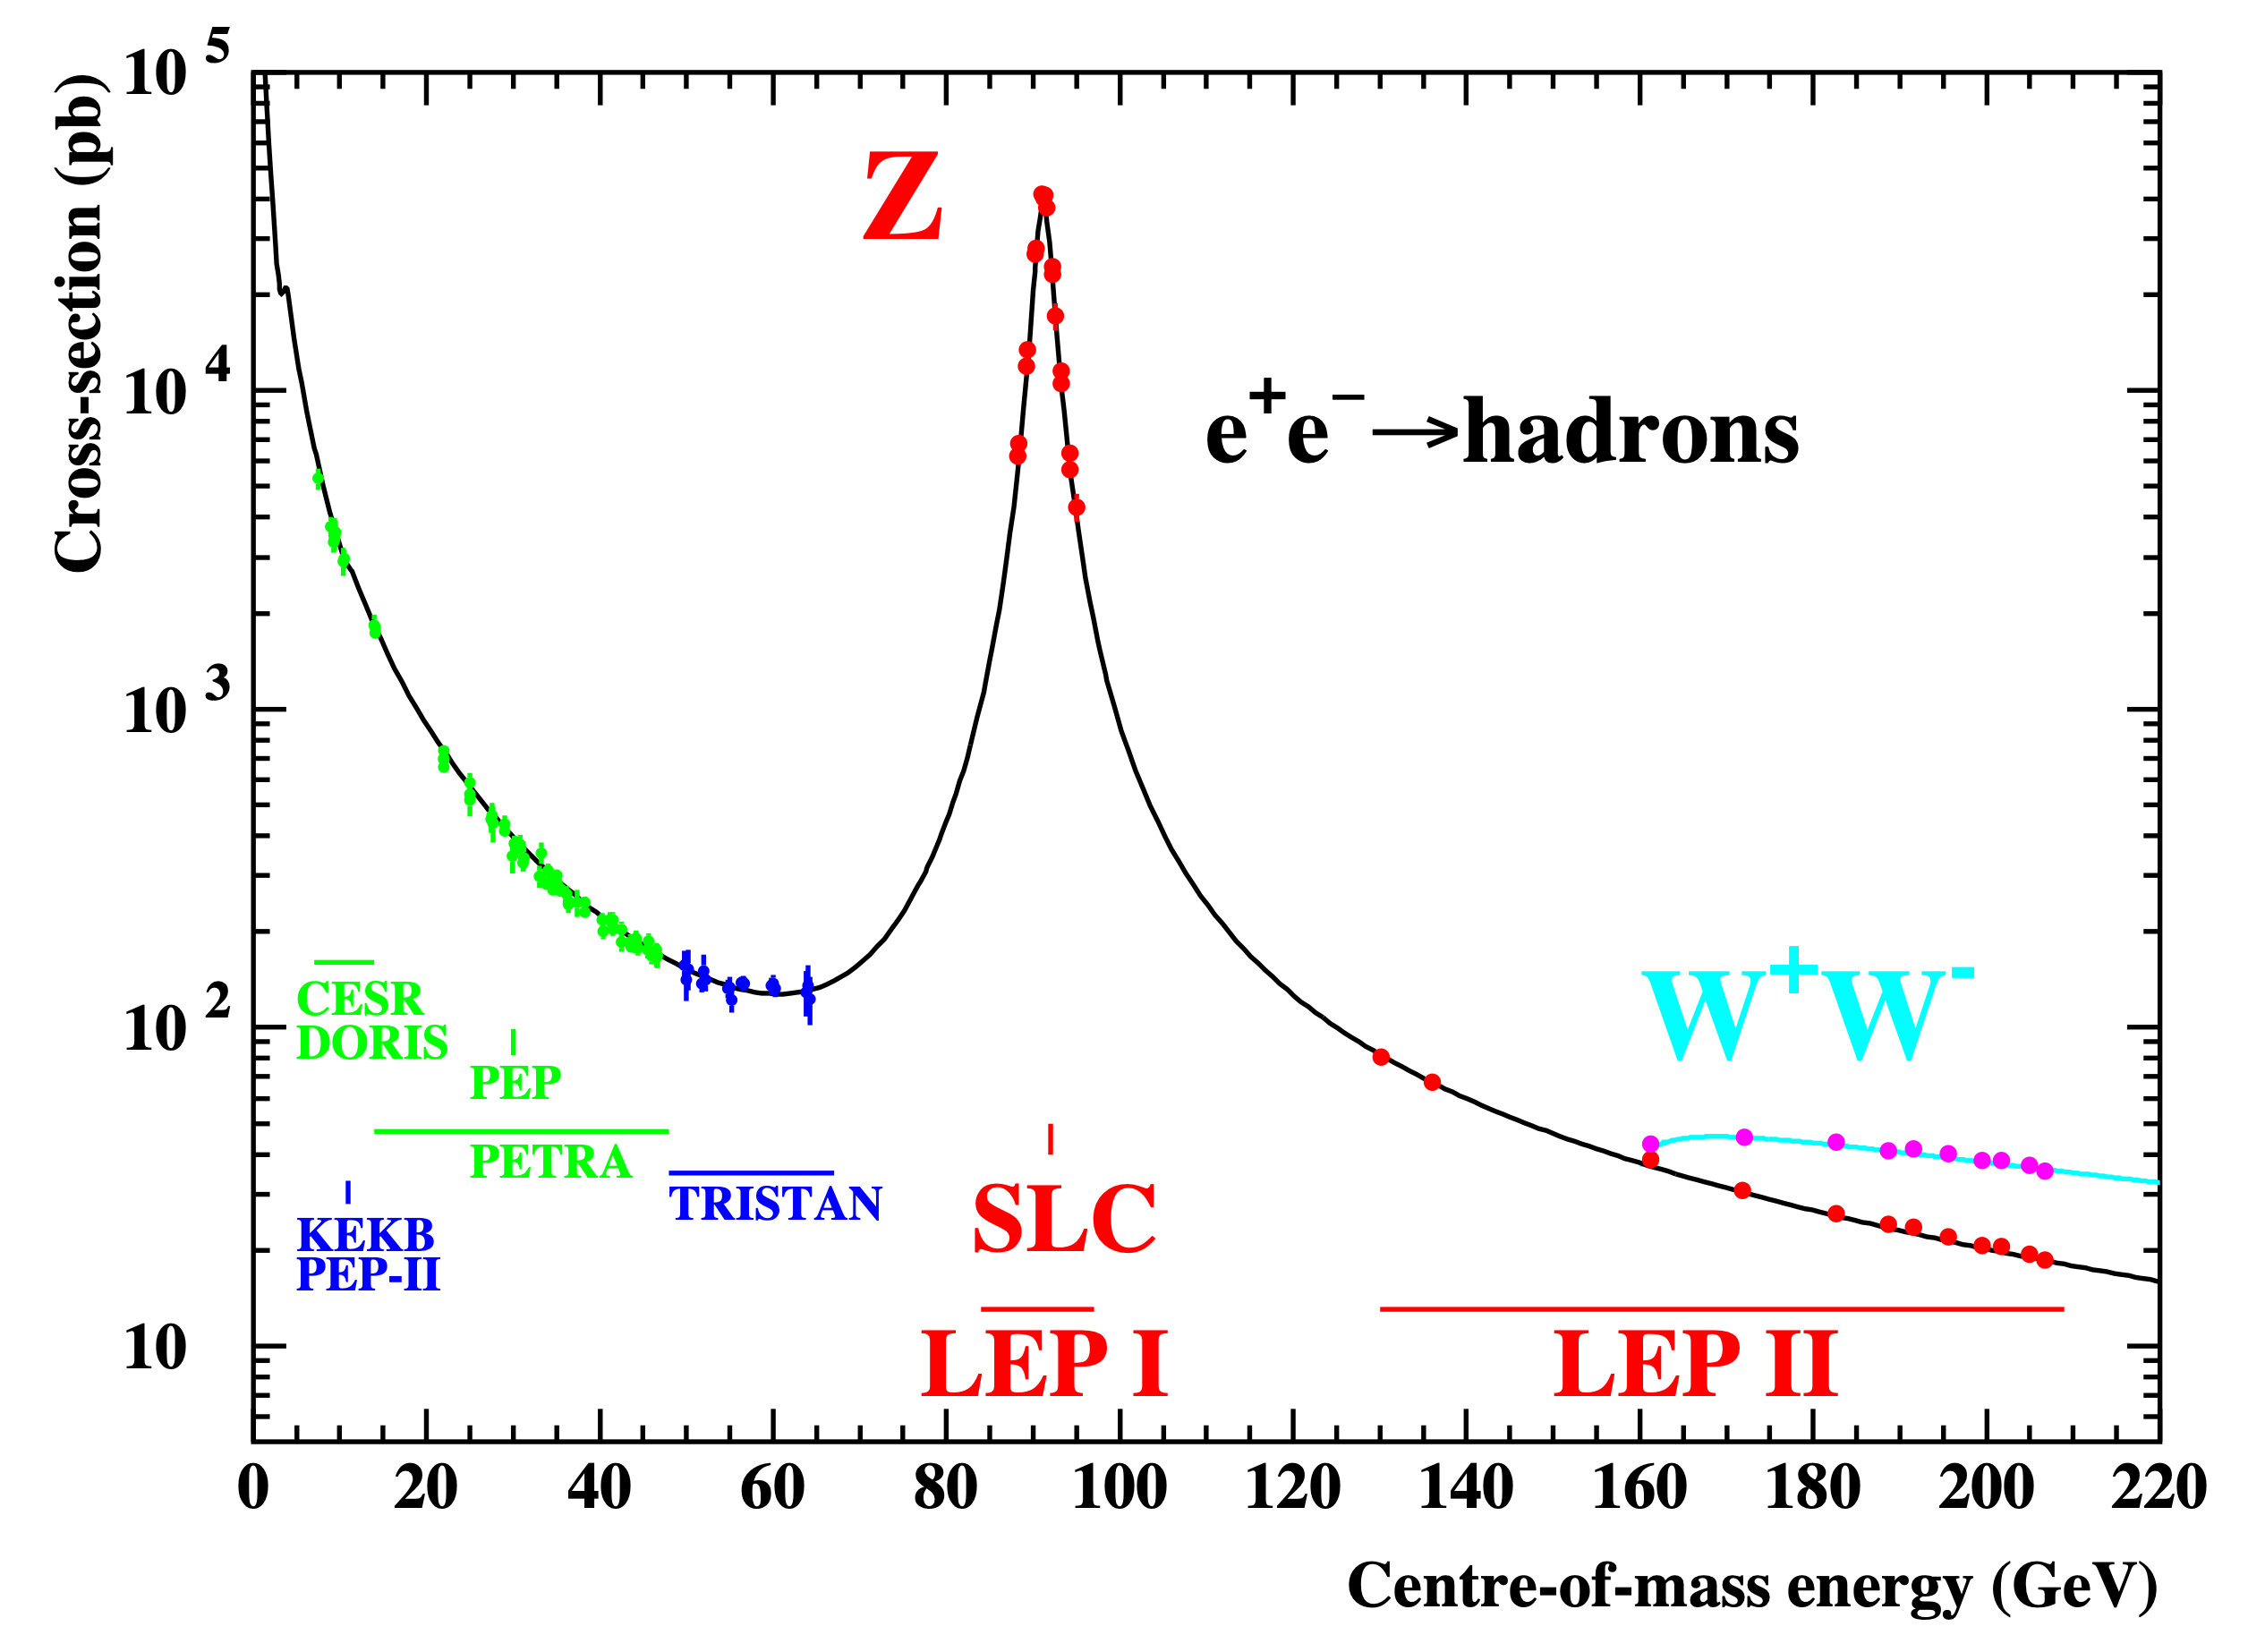
\includegraphics[width=0.8\textwidth]{figures/01-SM-02-QFT/eezpeak}
	\caption{Cross section for $e^+e^- \rightarrow$ hadron scattering as a function of $\sqrt{s}$ with a clear resonance at the $Z$ boson mass, reproduced from Ref.~\cite{ALEPH:2005ab}.}
	\label{fig:01_qft_interactions_eezpeak}
\end{figure}


\subsubsection{The classical limit and the Yukawa potential}

It is important to check our QFT recovers classical physics in the appropriate limit.
It will also be useful to translate the somewhat abstract idea of amplitudes to the familiar concepts of forces and potentials.
We will do so by considering the nonrelativistic limit ($\abs{\cvec{p}} \ll M$) of our above amplitudes and using the Born approximation relating the scattering amplitude between two particles to the potential between them $U(\cvec{r})$:
\begin{equation}
	\label{eq:01_qft_interactions_born}
	\mathcal M = \braket{\cvec{p}_f|U(\cvec{r})|\cvec{p}_i} = -i \int U(\cvec{r}) e^{i(\cvec{p}_f - \cvec{p}_i)\cdot\cvec{r}} d^3r,
\end{equation}
where $\cvec{r}$ is the displacement between the particles.

First, let us consider what this potential would be classically.
The static Klein-Gordon equation for a delta-function source:
\begin{equation}
	\label{eq:01_qft_interactions_static_kg}
	(\nabla^2 - m^2) \phi(\cvec{r}) = \delta^3(\cvec{r}),
\end{equation}
can be found via the Fourier transform to be:
\begin{equation}
	\label{eq:01_qft_interactions_static_kg_solution}
	\phi(\cvec{r}) =  \cfrac{e^{-mr}}{4\pi r}.
\end{equation}
We can interpret this to be the profile of $\phi$ around a nucleon (the delta function source), and thus conversely the potential felt by another nucleon via the meson and the Yukawa interaction, under the assumption $M \gg m$.
This is entirely analogous to gauge potential $A_0$ in electrostatics generated by a $\delta$-function source acting as the electric potential for a test charge.

Going back to our amplitude for nucleon-antinucleon scattering, the $s$-channel diagram vanishes in the nonrelativistic limit (which essentially means it does not have a simple classical interpretation), while the $t$-channel diagram actually stays the same:
\begin{equation}
	\label{eq:01_qft_interactions_na_scattering_nr}
	i \mathcal M = -(-ig)^2 \cdot \cfrac{1}{\abs{\cvec{p}_f - \cvec{p}_i}^2 - m^2}.
\end{equation}
Plugging this into the LHS of Eq.~\ref{eq:01_qft_interactions_born} and inverting the RHS integral gives us:
\begin{equation}
	\label{eq:01_qft_interactions_yukawa_potential}
	U(\cvec{r}) = -\cfrac{g^2}{4M^2} \cdot \cfrac{e^{-mr}}{4\pi r}.
\end{equation}
This is exactly the classical potential we found in Eq.~\ref{eq:01_qft_interactions_static_kg_solution}!
It is weighted by the coupling constant $g$ and $M$ to get the correct dimensions, and with a minus sign telling us potential is attractive.

Thus, we are able to reproduce Newtonian forces from the nonrelativisic limit of QFT.
We also have the new interpretation of forces as simply manifestations of interactions in the Lagrangian, occurring through the exchange of virtual particles.

This potential is called the \textit{Yukawa potential}, describing a force mediated by a massive boson.
As expected, in the limit $m \rightarrow 0$, we recover the familiar $1/r$ Coulomb potential, which is mediated by the massless photon.
We can check that we obtain the same potential for nucleon-nucleon scattering and, more generally, that all forces mediated by scalars are attractive.
In fact, this is true for spin-2 particles as well, which is why gravity is universally attractive!
On the other hand, forces mediated by spin-1 particles, such as EM, can be either attractive or repulsive, with the charges of the particles involved determining the sign of each diagram.
See e.g. Zee QFT~\cite{Zee:2003mt} Chapter I.5 for a useful discussion.


\subsubsection{Fourth-order diagrams and loops}

So far, we have only considered \textit{tree-level} diagrams, the simplest to calculate.
This is in contrast to diagrams with \textit{loops}, which can occur at higher order in perturbation theory.
For example, at fourth-order we can have diagrams like those in Figure~\ref{fig:01_qft_interactions_feynman_loops} for nucleon scattering. 

Such diagrams contribute integrals over the loop momentum $k$ to the matrix element, which can notoriously diverge.
To deal with this requires a process called \textit{renormalization}, which, briefly, involves defining a cut-off energy scale $\Lambda$ for these integrals, beyond which we claim the theory is invalid.
Experimentally, the main consequence is that physical parameters like the mass of particles and coupling constants in fact depend on the energy scale at which they are measured!

\begin{figure}[ht]
	\centering
	\captionsetup{justification=centering}
	\begin{tikzpicture}
		\begin{feynman}
			\vertex (a);
			\vertex [below=1cm of a] (c);
			\vertex [below=1.2cm of c] (d);
			\vertex [below=1cm of d] (b);
			\vertex [above left=of a] (i1);
			\vertex [below left=of b] (i2);
			\vertex [above right=of a] (f1);
			\vertex [below right=of b] (f2);
			\diagram* {
				(a) -- [scalar, edge label={\footnotesize$k_1$}] (c),
				(d) -- [scalar, edge label={\footnotesize$k_3$}] (b),
				(i1) -- [fermion, edge label'={\footnotesize$q_{i1}$}] (a),
				(i2) -- [fermion, edge label={\footnotesize$q_{i2}$}] (b),
				(a) -- [fermion, edge label'={\footnotesize$q_{f1}$}] (f1),
				(b) -- [fermion, edge label={\footnotesize$q_{f2}$}] (f2),
				(c) -- [fermion, half left, edge label'={\footnotesize$k_2$}] (d),
				(d) -- [fermion, half left] (c),
			};
		\end{feynman}
	\end{tikzpicture}
	\caption{An example of a higher-order scattering diagram with a ``loop''.}
	\label{fig:01_qft_interactions_feynman_loops}
\end{figure}

\subsection{Decay rates and cross sections}
\label{sec:01_qft_interactions_decay}

In this section, we translate our S-matrix elements to physical observables: cross sections and decay rates.

\subsubsection{Cross section}

Classically for a scattering experiment, the number of particles scattered $N$ is related to the cross sectional area $\sigma$ as:
\begin{equation}
	\label{eq:01_qft_interactions_cross_section_classical}
	N = \sigma T \Phi,
\end{equation}
where $T$ is the total time and $\Phi$ is the flux of incoming particles (number of incoming particles per unit area and unit time).
In QM, we define the cross section $\sigma$ similarly, but in terms of the probability of scattering $P$ instead of $N$:
\begin{equation}
	\label{eq:01_qft_interactions_cross_section_qm}
	\sigma = \frac{P}{\Phi T}.
\end{equation}
This is a more abstract quantity in QM, but it still has units of area.
The number of scattering events $N$ is related to $\sigma$ by a factor we call the \textit{luminosity} $L$:
\begin{equation}
	\label{eq:01_qft_interactions_cross_section_luminosity}
	N = \sigma L.
\end{equation}
Here, we simply consider this the definition of luminosity, but for a collider, for example, it can be derived from the properties of the input particle beams  (as will be discussed in Part~\ref{part:epp}).
Often, we are interested in the \textit{differential cross section} $d\sigma$ with respect to kinematic variables like the solid angle $\Omega$ or energy, so we write:
\begin{equation}
	\label{eq:01_qft_interactions_cross_section_differential}
	d\sigma = \frac{dP}{\Phi T}.
\end{equation}

As in QM, this probability $P$ is proportional to the square of the amplitude $|\braket{f|S|i}|^2$:
\begin{equation}
	\label{eq:01_qft_interactions_cross_section_probability}
	dP = \frac{\abs{\braket{f|S|i}}^2}{\braket{f|f}\braket{i|i}}\, d\Pi,
\end{equation}
where $\braket{f|f}$ and $\braket{i|i}$ are the normalization factors for the final and initial states (they are not equal to $1$ as discussed in Section~\ref{sec:01_qft_quantization_propagators}), and $d\Pi$ is the differential region of final state momenta.

For the case of two incoming particles (which is what is most relevant for this dissertation), we can put all of this together to obtain the relation between differential cross section and the matrix element $\mathcal M$:
\begin{equation}
	\label{eq:01_qft_interactions_cross_section_matrix_element}
	d\sigma = \frac{1}{(2E_1)(2E_2)\abs{\cvec{v}_1 - \cvec{v}_2}} \abs{\mathcal M}^2 d\Pi_\mathrm{LIPS},
\end{equation}
where $E_1$ and $E_2$ are the energies of the incoming particles, $\cvec{v}_1$ and $\cvec{v}_2$ are their velocities, and $d\Pi_\mathrm{LIPS}$ is called the Lorentz-invariant phase space of the final state momenta:
\begin{equation}
	\label{eq:01_qft_interactions_cross_section_lips}
	d\Pi_\mathrm{LIPS} = (2\pi)^4 \delta^{(4)}(\Sigma p) \prod_{\mathrm{final\ states}\ j} \frac{d^3p_j}{(2\pi)^3} \frac{1}{2E_j}
\end{equation}

For the case of $2 \rightarrow 2$ scattering, in the COM frame, this simplifies considerably:
\begin{equation}
	\label{eq:01_qft_interactions_cross_section_com}
	\bigg(\frac{d\sigma}{d\Omega}\bigg)_\mathrm{CM} = \frac{1}{64\pi^2E_\mathrm{CM}^2}\, \frac{\abs{\cvec{p}_f}}{\abs{\cvec{p}_i}} \abs{\mathcal M}^2 \theta(E_\mathrm{CM} - m_3 - m_4),
\end{equation}
and even more so when the all four masses are equal:
\begin{equation}
	\label{eq:01_qft_interactions_cross_section_com_equal_mass}
	\bigg(\frac{d\sigma}{d\Omega}\bigg)_\mathrm{CM} = \frac{1}{64\pi^2E_\mathrm{CM}^2}\, \abs{\mathcal M}^2.
\end{equation}

% For nucleon-nucleon scattering in the COM frame, for example, we have (at tree level):
% \begin{equation}
% 	\label{eq:01_qft_interactions_nn_scattering_cross_section}
% 	\begin{split}
% 		\bigg(\frac{d\sigma(\theta)}{d\Omega}\bigg)_\mathrm{CM} &= \frac{g^4}{64\pi (2E)^2} \left(\frac{1}{t - m^2} + \frac{1}{u - m^2}\right)^2 \\
% 		&= \frac{g^4}{64\pi (2E)^2} \left[\frac{1}{2p^2(1 - \cos\theta) - m^2} + \frac{1}{2p^2(1 + \cos\theta) - m^2}\right]^2,
% 	\end{split}
% \end{equation}
% where we used the expressions for $t$ and $u$ for a collision along the z-axis from Eq.~\ref{eq:01_qft_interactions_mandelstam_com}.

\subsubsection{Decay rate}

The other type of process we are interested in are decays.
The decay rate $\Gamma$ is simply the probability of decay per unit time:
\begin{equation}
	\label{eq:01_qft_interactions_decay_rate}
	\Gamma =  \frac{P}{T}.
\end{equation}
Using our expression for $P$ from above and simplifying, we find:
\begin{equation}
	\label{eq:01_qft_interactions_differential_decay_rate}
	d\Gamma = \frac{1}{2m} \abs{\mathcal M}^2 d\Pi_\mathrm{LIPS},
\end{equation}
in the rest frame of the decaying particle, where $m$ is its mass.
If multiple decays of the same particle are possible, we sum over the final states in the phase space integral.
The total $\Gamma$ is then called the \textit{width} of the particle, and $1/\Gamma \equiv \tau$ is its half-life.

For our simple meson decay $\phi \rightarrow \psi^\dagger\psi$, we have at tree level:
\begin{equation}
	\label{eq:01_qft_interactions_decay_rate_meson_decay}
	d\Gamma = \frac{g^2}{2m} d\Pi_\mathrm{LIPS} \quad \Rightarrow \quad \Gamma = \frac{g^2}{32\pi m} \left(1 - \frac{4M^2}{m^2}\right)^{1/2},
\end{equation}
where we performed the integral over $d\Pi_\mathrm{LIPS}$ (see Ref.~\cite{XianyuPSSolutions} 4.2).
This is in fact not too far off the expression for the decay width of the Higgs boson to fermions.
What we are missing of course is that fermions are spin-$\cnicefrac{1}{2}$ particles, and we need to sum over their spin states.
Fermions are described by spinor field theory, detailed in Appendix~\ref{sec:01_qft_spinors}.

\section{Gauge theories}
\label{sec:01_qft_gt}

% \begin{center}
% 	\centering
{
	\noindent
	\textit{Nature seems to take advantage of the simple mathematical representations of the symmetry laws. 
	When one pauses to consider the elegance and the beautiful perfection of the mathematical reasoning involved and contrast it with the complex and far-reaching physical consequences, a deep sense of respect for the power of the symmetry laws never fails to develop.} --- C. N. Yang
}
% \end{center}

\

So far, we have discussed spin-$0$ scalar bosons (and the spin-$\frac{1}{2}$ fermions in Appendix~\ref{sec:01_qft_spinors}); the last set of SM particles are the spin-$1$ \textit{gauge bosons}.
These are the particles which mediate all three fundamental forces in the SM: electromagnetism, the weak force, and the strong force.
Fortunately, compared to spinors, they live in the simpler and familiar vector representation of the Lorentz group.

On the other hand, they are intrinsically tied to a unique type of internal, \textit{local}, symmetry in QFT: \textit{gauge symmetry}.
Unlike, say, Lorentz or spacetime translation invariance, this is not a fundamental physical symmetry of nature, and is not associated with any consrervation law.
Instead, it simply describes a redundancy in our mathematical formulation of the gauge theory, stemming from the fact that the vector fields used to describe the gauge bosons have more degrees of freedom (DoFs) than the physical particles themselves.
The DoFs are thereby reduced by identifying fields related by a gauge symmetry transformation to be the same physical state, known as the principle of \textit{gauge invariance}.
This is entirely analogous to requiring that a change of coordinate system not affect the physics.
A deeper discussion of the motivations behind gauge invariance can be found in Appendix~\ref{sec:01_qft_gt_why}.
% In this section, we first discuss the motivations for gauge invariance in QFT in Section~\ref{sec:01_qft_gt_why}.

In this section, we first introduce the simplest gauge boson, the photon, and its associated \UU[1] gauge symmetry in Section~\ref{sec:01_qft_gt_maxwell}.
Coupling this to matter and quantizing the theory gives us QED, the relativistic quantum theory of electromagnetism (Section~\ref{sec:01_qft_gt_qed}).
We then generalize this to, and quantize, non-abelian gauge theories, known as Yang-Mills theories, in Sections~\ref{sec:01_qft_gt_yangmills} and~\ref{sec:01_qft_gt_ymquant}, respectively.
We conclude with a discussion of renormalization and the \textit{running} of coupling constants in Section~\ref{sec:01_qft_gt_asymptotic}.


\subsection{Maxwell Theory}
\label{sec:01_qft_gt_maxwell}

Gauge symmetries are a generalization of internal global symmetries, such as the \UU[1] symmetry from Section~\ref{sec:01_qft_classical_symmetries}, to a \textit{local} symmetry, where the symmetry transformation can be a function of spacetime.
We are most familiar with this concept from classical E\&M, in which Maxwell's laws are invariant under transformations of the $4$-vector potential $A_\mu = (\phi, \cvec{A})$ of the form:
\begin{equation}
	\label{eq:01_qft_gt_maxwell_gauge}
	A_\mu(x) \rightarrow A_\mu(x) + \frac{1}{e}\partial_\mu\alpha(x),
\end{equation}
for an arbitrary function $\alpha(x)$, where $e$ is a conventional constant that we will soon interpret as the coupling constant of the theory.
% Remarkably, once quantized, $A_\mu$ represents the photon field.

Recall that $A_\mu$ is related to the electric and magnetic fields, $\cvec{E}$ and $\cvec{B}$, by:
\begin{equation}
	\label{eq:01_qft_gt_maxwell_fields}
	\cvec{E} = -\nabla\phi - \partial_t\cvec{A}, \qquad \cvec{B} = \nabla\times\cvec{A},
\end{equation}
and the Maxwell equations can be derived from the Lagrangian:
\begin{equation}
	\label{eq:01_qft_gt_maxwell_lagrangian}
	\mathcal L = -\frac{1}{4}F_{\mu\nu}F^{\mu\nu},
\end{equation}
where
\begin{equation}
	\label{eq:01_qft_gt_maxwell_field_strength}
	F_{\mu\nu} = \partial_\mu A_\nu - \partial_\nu A_\mu
\end{equation}
is the \textit{field strength} tensor.
One can confirm that (1) $F_{\mu\nu}$ and, hence, the Lagrangian is invariant under the gauge transformation in Eq.~\ref{eq:01_qft_gt_maxwell_gauge}, and (2) the resulting E-L EOMs are exactly the homogeneous Maxwell equations.
Thus, classical E\&M was our earliest and simplest gauge theory, although the significance and generalization of gauge invariance only became clear with the advent of QFT.

Gauge invariance significantly restricts the possible terms in the Lagrangian (and thus considerably simplifies the theory).
Notably, mass terms like $m^2A_\mu^2$ \textit{violate} gauge invariance, which is why gauge bosons are necessarily massless, without something special like the Higgs mechanism (Section~\ref{sec:01_qft_higgs}).
As discussed in Appendix~\ref{sec:01_qft_gt_why}, gauge invariance also ensures the renormalizability of the theory and reduces the DoFs of $A_\mu$ such that, once quantized, we can identify it as the photonic field.

% Finally, note that our Lagrangian contains terms of the form $(\partial_\mu A_\nu)^2$; hence, $A_\mu$ (and all spin-$1$ fields) have dimension $1$.

\subsubsection{Interactions with scalars}

The \UU[1] nature of the gauge transformation becomes more apparent when we try to couple the photon to other particles.
Note that our Lagrangian above contains terms of the form $(\partial_\mu A_\nu)^2$ so $A_\mu$ (and indeed all spin-$1$ fields) have dimension $1$.

% \subparagraph{Coupling to scalars}
Let us consider a scalar field $\phi$: we can write renormalizable, scalar terms like $A_\mu^2\phi^2$ and $A_\mu \phi\partial_\mu\phi$; however, they do not look gauge invariant.
To make them so, we must require that $\phi$ \textit{also} transforms under the same gauge transformation in a way that compensates the change in $A_\mu$.

The simplest way is to take $\phi$ to be a \textit{complex} scalar field and ``promote'' its inherent global \UU[1] symmetry to a local one:
\begin{equation}
	\label{eq:01_qft_gt_maxwell_scalar_gauge}
	\phi(x) \rightarrow e^{iQ_\phi\alpha(x)}\phi(x),
\end{equation}
where we say $Q_\phi$ represents the charge of $\phi$ under the \UU[1] symmetry.\footnote{Note that such a transformation is not possible with a \textit{real} field, which necessarily has $0$ charge and does not couple with the photon.}
% Since we will not be discussing more than one interacting field until the next chapter, we will henceforth take $Q = 1$ for simplicity.
We can then define the \textit{covariant derivative} acting on $\phi$ as:\footnote{As discussed above, this is the same concept as the covariant derivative in GR, with the gauge field $A_\mu$ acting as a connection on a \UU[1] fiber bundle analogously to the Levi-Civita connection between tangent bundles.
Essentially, it encodes the change in the local phase of $\phi$ across spacetime (see Peskin and Shroeder~\cite{Peskin:1995ev} Chapter 15.1 for a nice derivation of this).
}
\begin{equation}
	\label{eq:01_qft_gt_maxwell_covariant_derivative}
	D_\mu\phi = (\partial_\mu - ieQ_\phi A_\mu)\phi,
\end{equation}
where $e$ is the same coupling constant from Eq.~\ref{eq:01_qft_gt_maxwell_gauge}.

One can check that $D_\mu\phi$ transforms under the gauge transformation as:
\begin{equation}
	\label{eq:01_qft_gt_maxwell_covariant_derivative_gauge}
	D_\mu\phi \rightarrow e^{iQ_\phi\alpha(x)}D_\mu\phi,
\end{equation}
meaning $(D_\mu\phi)^\dagger D^\mu\phi$ provides us with a gauge invariant interaction term for the Lagrangian.
Thus, we have a gauge invariant \textit{scalar} QED Lagrangian:
\begin{equation}
	\label{eq:01_qft_gt_maxwell_scalar_lagrangian}
	\mathcal L = -\frac{1}{4}F_{\mu\nu}F^{\mu\nu} + (D_\mu\phi)^\dagger D^\mu\phi - m^2\abs{\phi}^2.
\end{equation}

Note that the commutator of the covariant derivative is in fact not a derivative at all, but proportional to the field strength tensor:
\begin{equation}
	[D_\mu, D_\nu]\phi = ([\partial_\mu, \partial_\nu] - ie[\partial_\mu, A_\nu] + ie[\partial_\nu, A_\mu])\phi = -ieF_{\mu\nu}\phi.
\end{equation}
Thus, we can define $F_{\mu\nu} \equiv \frac{i}{e}[D_\mu, D_\nu]$, which will prove useful for non-abelian gauge symmetries later in this section.
% By definition, higher order covariant derivatives transform the same way as the first order, meaning $F_{\mu\nu}$ transforms as $F_{\mu\nu} \rightarrow 

Generally, we choose the normalization $Q_e = -1$ for the electron field, so $e$ becomes our familiar elementary charge (in natural units) and $\alpha\equiv\cnicefrac{e^2}{4\pi} \approx \cnicefrac{1}{137}$ is the famous dimensionless fine structure constant.\footnote{Technically, this value varies with our energy scale, as we will discuss in Section~\ref{sec:01_qft_gt_asymptotic}, and $\cnicefrac{1}{137}$ is its asymptotic value at low energies.}

\subsubsection{Interactions with spinors}

The case for spinors is not so different. 
The definition of the covariant derivative remains the same, so combining the ``covariant'' Dirac Lagrangian with the free photonic yields the QED Lagrangian:
\begin{equation}
	\label{eq:01_qft_gt_maxwell_qed_lagrangian}
	\mathcal L = -\frac{1}{4}F_{\mu\nu}F^{\mu\nu} + \bar\psi(i\cslashed D - m)\psi.
\end{equation}
This is in fact the most general possible Lorentz-invariant, renormalizable, $P$-symmetric Lagrangian for a spinor field with a \UU[1] gauge symmetry, and can thus be derived from the requirement of gauge invariance alone (as done in e.g. Peskin and Shroeder~\cite{Peskin:1995ev} Chapter 15.1).
This is a general feature of the SM: every possible term permitted by gauge invariance and the usual physical requirements of Lorentz invariance etc. is included in the Lagrangian (with one possible exception that forms the basis for the strong CP problem~\cite{Wu:1991rw,Mannel:2007zz}).

Expanding out the Lagrangian, we have:
\begin{equation}
	\label{eq:01_qft_gt_maxwell_qed_lagrangian_expanded}
	\mathcal L = -\frac{1}{4}F_{\mu\nu}F^{\mu\nu} + \bar\psi(i\gamma^\mu\partial_\mu - m)\psi - e\bar\psi\gamma^\mu\psi A_\mu,
\end{equation}
where we see this interaction term is simply $-ej^\mu A_\mu$ with $j^\mu = \bar\psi\gamma^\mu\psi$ the conserved current associated with the \textit{global} \UU[1] symmetry we found in Section~\ref{sec:01_qft_spinors_lagrangian}.
One can check that the E-L EOMs for $A_\mu$ now correspond to the \textit{inhomogeneous} Maxwell equations with a source term $J_\mu \equiv -ej_\mu$:
\begin{equation}
	\label{eq:01_qft_gt_maxwell_qed_inhomo_eqs}
	\partial_\mu F_{\mu\nu} = J_\nu,
\end{equation}
reproducing our beloved E\&M from this field theory formulation!
% \TODO{We will discuss Feynman diagrams and important processes in the next chapter?}

\subsection{Quantum electrodynamics}
\label{sec:01_qft_gt_qed}

The quantized version of the above is what we call \textit{quantum electrodynamics} (QED): the QFT of electromagnetic interactions.
It has proven an extraordinarily successful theory, serving as a model for the remainder of the SM as well as theories for condensed matter phenomena.

The exact path to quantizing $A_\mu$ depends on the choice of gauge.
We will forego those details and simply use physical intuition --- namely, that the photon has only two physical, transverse polarizations --- to motivate the result:
\begin{equation}
	\label{eq:01_qft_gt_maxwell_quantization}
	A_\mu(x) = \int \frac{d^3p}{(2\pi)^3} \frac{1}{\sqrt{2E_p}} \sum_{\lambda=1}^2 \left(\epsilon_\mu^\lambda(p)\hat a^\lambda_p e^{-ip\cdot x} + \epsilon_\mu^{\lambda*}(p) \hat a^{\lambda\dagger}_p e^{ip\cdot x}\right),
\end{equation}
where $\epsilon_\mu^\lambda(p)$ are the two transverse polarization basis vectors and $a_p^\lambda$ and $a^{\lambda\dagger}_p$ are the photon annihilation and creation operators.

The photon propagator depends as well on the choice of gauge.
Expanding the homogeneous photon EOM, Eq.~\ref{eq:01_qft_gt_maxwell_qed_inhomo_eqs}, gives:
\begin{equation}
	\label{eq:01_qft_gt_maxwell_photon_eom_psapce}
	\partial_\mu\partial^\mu A_\nu - \partial_\nu\partial_\mu A^\mu = J_\nu,
\end{equation}
which in momentum space becomes:
\begin{equation}
	\label{eq:01_qft_gt_maxwell_photon_eom_momentum}
	(-p^2 \eta_{\mu\nu} + p_\mu p_\nu) A_\mu  = J_\nu.
\end{equation}
Recall that the propagator is the inverse of the operator on the LHS for a delta-function source; however, due to the redundant DoFs of $A_\mu$, this is not directly invertible without first fixing a gauge.

The cleanest way to do so is to add a ``Lagrange multiplier'' term representing the gauge fixing condition to the Lagrangian.
The most common choice is the \textit{Lorenz gauge}, $\partial_\mu A^\mu = 0$, which makes Lorentz-invariance manifest and to enforce which we can include the term $-\frac{1}{2\xi}(\partial_\mu A^\mu)^2$.
One can confirm that the EOM for $\xi$ is exactly the Lorenz gauge condition.
Inverting the new EOM for $A_\mu$ gives us the (Feynman) photon propagator:
\begin{equation}
	\label{eq:01_qft_gt_maxwell_photon_propagator}
	\Delta_{\mu\nu}(p) = \frac{-i}{p^2 + i\epsilon}\left[ \eta_{\mu\nu} + (1-\xi)\frac{p_\mu p_\nu}{p^2} \right].
\end{equation}
This is called the $R_\xi$ gauge and different values of $\xi$ correspond to different propagators, each with their own advantages and disadvantages for calculations.
In QED, we typically take $\xi = 1$, called the Feynman-'t Hooft gauge, for simplicity:
\begin{equation}
	\label{eq:01_qft_gt_maxwell_photon_propagator_feynman}
	\Delta_{\mu\nu}(p) = \frac{-i \eta_{\mu\nu}}{p^2 + i\epsilon}.
\end{equation}

\begin{definition}
	\label{def:01_qft_gt_maxwell_feynman}
	With this, we can write down the Feynman rules for QED, with spinor ($\alpha$, $\beta$) and $4$-vector ($\mu$, $\nu$) indices labeled explicitly for clarity:
	% feynman rules for QED
\begin{enumerate}
	\item Vertices: \qquad
	\begin{tikzpicture}[baseline={(current bounding box.center)}]
		\begin{feynman}[small]
			\vertex (a) {$\mu$};
			\vertex [right=of a] (b);
			\vertex [above right=of b] (f1) {$\alpha$};
			\vertex [below right=of b] (f2) {$\beta$};
			\diagram* {
				(a) -- [boson] (b),
				(b) -- [fermion] (f1),
				(b) -- [anti fermion] (f2),
			};
		\end{feynman}
	\end{tikzpicture}
	$ = -i e \gamma^\mu_{\alpha\beta}$ \\[1em]
	\item Internal lines (propagators) \\[1em]
	\qquad\qquad Fermions: \qquad
	\begin{tikzpicture}[baseline={([yshift=-0.7ex]current bounding box.center)}]
		\begin{feynman}
			\vertex (a) {$\alpha$};
			\vertex [right=of a] (b) {$\beta$};
			\diagram* {
				(a) -- [fermion, edge label={\footnotesize$q$}] (b),
			};
		\end{feynman}
	\end{tikzpicture}
	\quad $\, = \bigg(\cfrac{i(\cslashed{q} + m)}{q^2 - M^2 + i\varepsilon}\bigg)_{\alpha\beta}$ 
    \\[1em]
    Photons: \qquad \;
	\begin{tikzpicture}[baseline={([yshift=-0.7ex]current bounding box.center)}]
		\begin{feynman}
			\vertex (a) {$\mu$};
			\vertex [right=of a] (b) {$\nu$};
			\diagram* {
				(a) -- [boson, edge label={\footnotesize$p$}] (b),
			};
		\end{feynman}
	\end{tikzpicture}
	\quad $\, = -i \cfrac{\eta_{\mu\nu}}{p^2 + i\epsilon}$ 
    \\[1em]
	\item External lines (on-shell particles)  \\
    % \\[1.5em]
    % % \hspace*{-\leftmargini}
    % \begin{minipage}{0.99\textwidth}
    \begin{tabbing}
    Incoming fermions: 
    \hspace*{1.5cm}
    \=
    \begin{tikzpicture}[baseline={([yshift=-0.8ex]current bounding box.center)}]
        \begin{feynman}
            \vertex (a) {$\alpha$};
            \vertex [right=of a] (b);
            \vertex [above right=of b] (f1);
            \vertex [below right=of b] (f2);
            \diagram* {
                (a) -- [fermion, momentum={\footnotesize$q, s$}] (b),
                (b) -- [fermion] (f1),
                (b) -- [boson] (f2),
            };
        \end{feynman}
    \end{tikzpicture}
    \hspace*{0.4cm}
    \=
    $ = u^s_\alpha(q)$
    \\[1.5em]
    Incoming antifermions: 
    \>
    \begin{tikzpicture}[baseline={([yshift=-0.8ex]current bounding box.center)}]
        \begin{feynman}
            \vertex (a) {$\alpha$};
            \vertex [right=of a] (b);
            \vertex [above right=of b] (f1);
            \vertex [below right=of b] (f2);
            \diagram* {
                (a) -- [anti fermion, momentum={\footnotesize$q, s$}] (b),
                (b) -- [anti fermion] (f1),
                (b) -- [boson] (f2),
            };
        \end{feynman}
    \end{tikzpicture}
    \>
    $ = \bar v^s_\alpha(q)$
    \\[1.5em]
    Outgoing fermions: 
    \>
    % \hspace*{1.5cm}
    \begin{tikzpicture}[baseline={([yshift=-0.8ex]current bounding box.center)}]
        \begin{feynman}
            \vertex (a);
            \vertex [right=of a] (b) {$\alpha$};
            \vertex [above left=of a] (f1);
            \vertex [below left=of a] (f2);
            \diagram* {
                (f1) -- [fermion] (a),
                (f2) -- [boson] (a),
                (a) -- [fermion, momentum={\footnotesize$q, s$}] (b),
            };
        \end{feynman}
    \end{tikzpicture}
    \>
    $ = \bar{u}^s_\alpha(q)$
    \\[1.5em]
    Outgoing antifermions: 
    \>
    % \hspace*{1.5cm}
    \begin{tikzpicture}[baseline={([yshift=-0.8ex]current bounding box.center)}]
        \begin{feynman}
            \vertex (a);
            \vertex [right=of a] (b) {$\alpha$};
            \vertex [above left=of a] (f1);
            \vertex [below left=of a] (f2);
            \diagram* {
                (f1) -- [anti fermion] (a),
                (f2) -- [boson] (a),
                (a) -- [anti fermion, momentum={\footnotesize$q, s$}] (b),
            };
        \end{feynman}
    \end{tikzpicture}
    \>
    $ = v^s_\alpha(q)$
    \\[1.5em]
    Incoming photons: 
    \>
    \begin{tikzpicture}[baseline={([yshift=-0.8ex]current bounding box.center)}]
        \begin{feynman}
            \vertex (a) {$\mu$};
            \vertex [right=of a] (b);
            \vertex [above right=of b] (f1);
            \vertex [below right=of b] (f2);
            \diagram* {
                (a) -- [boson, momentum={\footnotesize$p, s$}] (b),
                (b) -- [fermion] (f1),
                (b) -- [anti fermion] (f2),
            };
        \end{feynman}
    \end{tikzpicture}
    \>
    $ = \epsilon^\lambda_\mu$
    \\[1.5em]
    Outgoing photons: 
    \>
    \begin{tikzpicture}[baseline={([yshift=-0.8ex]current bounding box.center)}]
        \begin{feynman}
            \vertex (a);
            \vertex [right=of a] (b) {$\mu$};
            \vertex [above left=of a] (f1);
            \vertex [below left=of a] (f2);
            \diagram* {
                (f1) -- [fermion] (a),
                (f2) -- [anti fermion] (a),
                (a) -- [boson, momentum={\footnotesize$p, s$}] (b),
            };
        \end{feynman}
    \end{tikzpicture}
    \>
    $ = \epsilon^{\lambda*}_\mu$
    \\
    \end{tabbing}
	\item Impose momentum conservation at each vertex.
	\item Integrate over the momentum $k$ flowing through each loop.
	\item Figure out the sign based on statistics. 
\end{enumerate}
	% QED has proven over the last century to be one of our most precise and successful theories;
	% we will look at some of its important processes in the next chapter.
\end{definition}

% \subsubsection{A scattering example and the Coulomb potential}

These Feynman rules can be applied to simple tree-level processes similarly to Yukawa theory (see Sections~\ref{sec:01_qft_interactions_feynman} and~\ref{sec:01_qft_spinors_feynman}).
These include several important processes such as electron-electron scattering $e^-e^- \rightarrow e^-e^-$ via a virtual photon, Compton scattering $\gamma e^- \rightarrow \gamma e^-$, electron-positron annihilation $e^+e^- \rightarrow \gamma\gamma$, and electron-positron (or Bhabha) scattering $e^+e^- \rightarrow e^+e^-$.
% We will discuss just one example, of electron-electron scattering $e^-e^- \rightarrow e^-e^-$, 
The former (and its variations with other charged particles) is what we generally experience as electromagnetism, and can recover the Coloumb potential in the non-relativistic limit.


\subsection{Yang-Mills Theory}
\label{sec:01_qft_gt_yangmills}

Following the remarkable success of QED and GR, a generalization of such gauge theories to \textit{non-abelian} symmetries was proposed by Chen Ning Yang and Robert Mills in 1953~\cite{Yang:1954ek}, today referred to as \textit{Yang-Mills} theories.
These theories picked up steam in the 1960s when the concept of spontaneous symmetry breaking was developed to give mass to the gauge bosons (Section~\ref{sec:01_qft_higgs}) and it was realized that both the weak and strong interactions can be described by \SU[2] and \SU[3] Yang-Mills theories, respectively.
They are hence a cornerstone of the SM, and we will now briefly outline their construction, generalizing the \UU[1] gauge symmetry from the previous section.
% Since then, Yang-Mills theories have become the cornerstone of the SM, with the electroweak and strong interactions described by \suu and \SU[3] Yang-Mills theories, respectively.
% We now briefly outline the generalization of \UU[1] gauge theories to these non-abelian gauge groups, leaving discussions of the many subtleties related to quantization and anomalies to dedicated texts such as Tong GT~\cite{TongGT} and Peskin and Shroeder~\cite{Peskin:1995ev}.

\subsubsection{Non-abelian gauge transformations}

In Yang-Mills theory, we allow non-gauge fields to transform locally under \textit{any} Lie group $G$, in an arbitrary representation $R$ of the group (generally, in the SM, $R$ is either the fundamental or trivial representation).
This means the fields $\psi$ are actually vectors of $\dim(R)$ (on top of their usual spinor or $4$-vector indices etc.), and transform as:
\begin{equation}
	\label{eq:01_qft_gt_yangmills_transformation}
	\psi(x) \rightarrow \psi'(x) = e^{i\alpha^a(x)T_R^a}\psi(x) \equiv V(x) \psi(x),
\end{equation}
where $T_R^a$ are the generators of $G$ in the representation $R$ and $V(x) = e^{i\alpha^a(x)T_R^a}$ is the gauge transformation.
To construct a $G$-invariant Lagrangian, we again need to define a covariant derivative with gauge fields $A_\mu^a$ connecting the local transformations of $\psi$ across spacetime:
\begin{equation}
	\label{eq:01_qft_gt_yangmills_dmu}
	D_\mu\psi = (\partial_\mu - igA_\mu^aT_R^a)\psi.
\end{equation}
Observe that we must have as many gauge fields as there are group generators to counter all possible gauge transformations $V(x)$; i.e., there are $\dim(G)$ $A_\mu$s, living in the \textit{adjoint} representation of $G$ (see Chapter~\ref{sec:01_symmetries_so3}).
The gauge field is often represented more conveniently as a ``Lie-algebra-valued'' field (i.e., as an object in the Lie algebra):
\begin{equation}
	\label{eq:01_qft_gt_yangmills_gauge_field}
	A_\mu \equiv A_\mu^aT^a.
\end{equation}

We can derive how $A_\mu$ transforms by requiring the covariant derivative to transform identically to $\psi$ (the same as in the abelian case):\footnote{For a detailed derivation see e.g. Ricardo Matheus' QFT Lectures~\cite{MatheusQFT} Part 34.}
\begin{equation}
	\label{eq:01_qft_gt_yangmills_dmu_transformation}
	D_\mu\psi \rightarrow D'_\mu\psi = (\partial_\mu - igA_\mu')V\psi \mustequal VD_\mu\psi(x),
\end{equation}
where $g$ is the coupling constant.
One can check this is satisfied for the transformed gauge field:
\begin{equation}
	\label{eq:01_qft_gt_yangmills_gauge_transformation_A}
	 A_\mu' = V A_\mu V^{-1} - \frac{i}{g}(\partial_\mu V)V^{-1}.
\end{equation}
For infinitesimal gauge transformations $V \simeq 1 + i\alpha^aT_R^a$, this can be written in terms of the components as:
\begin{equation}
	\label{eq:01_qft_gt_yangmills_gauge_transformation_A_infinitesimal}
	 A_\mu^{'a}T^a = A_\mu^aT^a + \frac{1}{g}\partial_\mu\alpha^aT^a + i A_\mu^a\alpha^b[T^b, T^a] = A_\mu^aT^a + \frac{1}{g}\partial_\mu\alpha^aT^a - f^{abc}A_\mu^a\alpha^bT^c,
\end{equation}
where $f^{abc}$ are the structure constants of the Lie algebra of $G$.
The second term represents the gauge transformation, same as in the abelian case, while the third term is new and is the transformation property for a field in the adjoint representation.
% In the abelian case, $f^{abc} = 0$ and we reproduce the \UU[1] transformation, Eq.~\ref{eq:01_qft_gt_maxwell_gauge}.

\subsubsection{The field strength tensor}

The final piece we need for the Lagrangian is a gauge-invariant kinetic term for the gauge fields, generalizing the electromagnetic field strength tensor $F_{\mu\nu}$.
We can construct this, as in the abelian case, using the commutator of covariant derivatives:
\begin{equation}
	\label{eq:01_qft_gt_yangmills_field_strength}
	F_{\mu\nu} \equiv \frac{i}{g}[D_\mu, D_\nu] = (\partial_\mu A_\nu^a - \partial_\nu A_\mu^a) - ig[A_\mu, A_\nu].
\end{equation}
Again, this reduces to the E\&M tensor for an abelian symmetry, where the commutator term is $0$.
In the non-abelian case, the commutator term adds new \textit{self-interaction} terms to the gauge fields.
One can check that $F_{\mu\nu}$ transforms as:
\begin{equation}
	\label{eq:01_qft_gt_yangmills_field_strength_transformation}
	F_{\mu\nu} \rightarrow V F_{\mu\nu} V^{-1},
\end{equation}
or, infinitesimally, in terms of components as:
\begin{equation}
	\label{eq:01_qft_gt_yangmills_field_strength_transformation_infinitesimal}
	F_{\mu\nu}^aT^a \rightarrow F_{\mu\nu}^aT^a + f^{abc}F_{\mu\nu}^b\alpha^cT^a,
\end{equation}
which we can recognize as the transformation of a field in the adjoint representation (Eq.~\ref{eq:01_qft_gt_yangmills_gauge_transformation_A_infinitesimal} without the gauge transformation term).

Clearly, for non-abelian theories, the field-strength tensor alone, or even $F_{\mu\nu}F^{\mu\nu}$, is no longer gauge-invariant; however, its \textit{trace} is:
\begin{equation}
	\label{eq:01_qft_gt_yangmills_trace_field_strength_transformation}
	\tr{F_{\mu\nu}F^{\mu\nu}} \rightarrow \tr{V F_{\mu\nu}V^{-1} V F^{\mu\nu} V^{-1}} = \tr{F_{\mu\nu}F^{\mu\nu}}
\end{equation}
using the cyclic property of the trace, providing us with a gauge-invariant kinetic term for the gauge fields.
In terms of components, this is:
\begin{equation}
	\label{eq:01_qft_gt_yangmills_trace_field_strength}
	\tr{F_{\mu\nu}F^{\mu\nu}} = F_{\mu\nu}^aF^{a\mu\nu}\, \tr{T^aT^a}
\end{equation}
The value of $\tr{T^aT^a}$ is a normalization constant that is conventionally chosen to be $\frac{1}{2}$ for the fundamental representation.
Expanding out $(F_{\mu\nu}^a)^2$ gives us cubic and quartic self-interaction terms for the gauge fields.

\subsubsection{The Yang-Mills Lagrangian}

Combining all of the above, we have the gauge-invariant Yang-Mills Lagrangian:
\begin{equation}
	\label{eq:01_qft_gt_yangmills_lagrangian}
	\mathcal L = -\frac{1}{2}\tr{F_{\mu\nu}F^{\mu\nu}} + \bar\psi(i\cslashed D - m)\psi,
\end{equation}
or, in explicit, component form:
\begin{equation}
	\label{eq:01_qft_gt_yangmills_lagrangian_explicit}
	\mathcal L = -\frac{1}{4}F_{\mu\nu}^aF^{a\mu\nu} + \bar\psi_i[\delta_{ij}(i\cslashed \partial_\mu - m) + g\cslashed A^aT_{ij}^a]\psi_j,
\end{equation}
where the indices $i$ and $j$ are running over the fermion fields in the representation $R$.
Note again that a mass term $m^2A_\mu^aA^{a\mu}$ would violate gauge invariance without the Higgs mechanism.

Interestingly, despite the extra self-interaction terms, there remains only one free parameter in the theory: the coupling constant $g$.
This is why the SM, despite its apparent complexity, has so few free parameters, particularly in the ``gauge sector'' (the majority of free parameters are related to couplings in the \textit{Higgs} sector).
It is also worth emphasizing that the primary difference \textit{physically} between abelian and non-abelian gauge theories is that the gauge bosons are charged under the gauge group in the latter (and, hence, self-interact).

% On the other hand, there is a new term which \textit{is} possible, 


\subsubsection{Quantum Yang-Mills Theory}
\label{sec:01_qft_gt_ymquant}

The form of the quantized gauge fields in Yang-Mills are similar to the \UU[1] case, except now with the extra adjoint representation indices.
The process of quantization and deriving the propagator, however, is considerably more involved for non-abelian theories.
The core idea of adding an $R_\xi$ gauge-fixing term to the Lagrangian is similar, but due to the gauge fields' non-trivial transformation property, the proper treatment necessitates the introduction of imaginary internal particles called \textit{Faddeev-Popov ghosts} to cancel gauge-dependent terms.
Somewhat similar to virtual particles, these ghosts are purely mathematical artifacts required to maintain gauge- and Lorentz-invariance of the quantized theory.
The full details of this process can be found in e.g. Peskin and Shroeder~\cite{Peskin:1995ev} Chapter 16; the upshot is simply some extra Feynman rules involving ghost particles in the theory.

The new Feynman rules for \textit{non-abelian Yang-Mills} theories are shown in Figure~\ref{fig:01_qft_gt_yangmills_feynman}.
The gauge bosons are conventionally referred to as ``gluons'' but these rules are general.
Note the cubic and quartic gauge boson vertices, as well as the ghost particle ($c$) diagrams, unique to non-abelian theories.
The phenomenology of Yang-Mills theories in the SM will be discussed in the next chapter.

\begin{figure}[ht!]
	\centering
	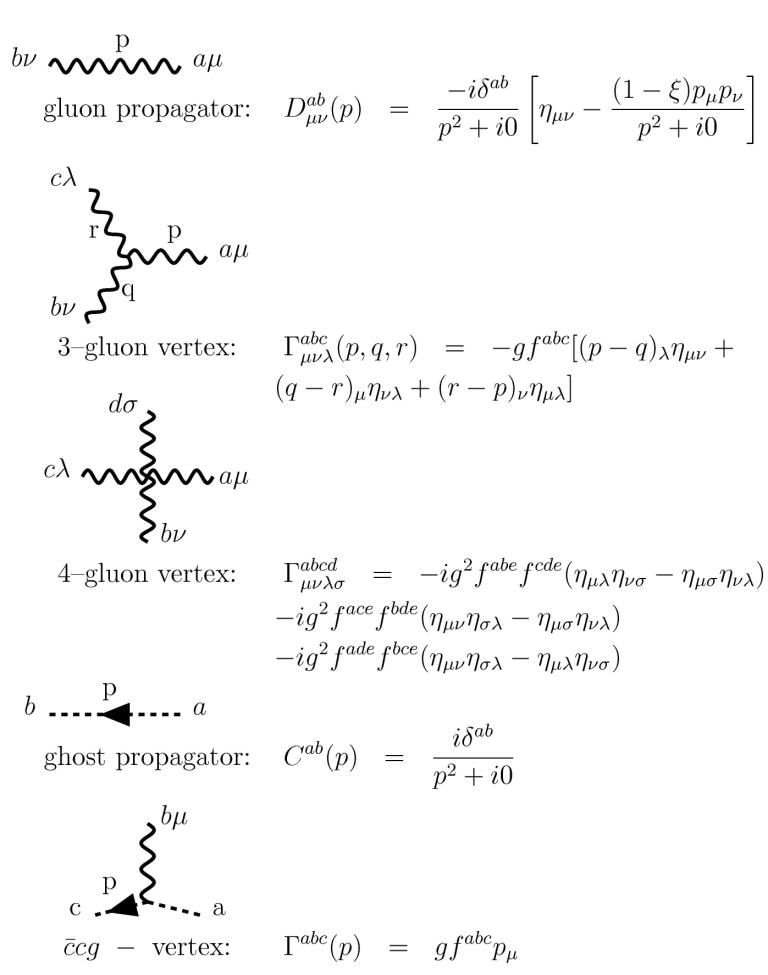
\includegraphics[width=0.8\textwidth]{figures/01-SM-02-QFT/Feynman/yangmills}
	\caption{Feynman rules unique to non-abelian Yang-Mills theories, reproduced from Ref.~\cite{enwiki:1243569653}.}
	\label{fig:01_qft_gt_yangmills_feynman}
\end{figure}


\subsection{Running couplings and asymptotic freedom}
\label{sec:01_qft_gt_asymptotic}

As discussed briefly in Section~\ref{sec:01_qft_interactions}, in order to handle divergences from higher order ``loop'' diagrams in perturbation theory, a class of mathematical techniques called \textit{renormalization} is employed.
A perhaps surprising physical consequence of this is that parameters of the theory are dependent on the energy scale at which they are probed.
Their dependence is described the \textit{renormalization group equations} or \textit{flow}.

The renormalization group is an extremely deep subject with applications in many areas of physics.
The most relevant result for us is the \textit{running} of the coupling constants in gauge theories --- i.e., the strength of the corresponding forces as a function of the energy scale.
This is shown for the relevant \UU[1], \SU[2], and \SU[3] gauge symmetries of the SM in Figure~\ref{fig:01_qft_running}.

\begin{figure}[ht]
	\centering
	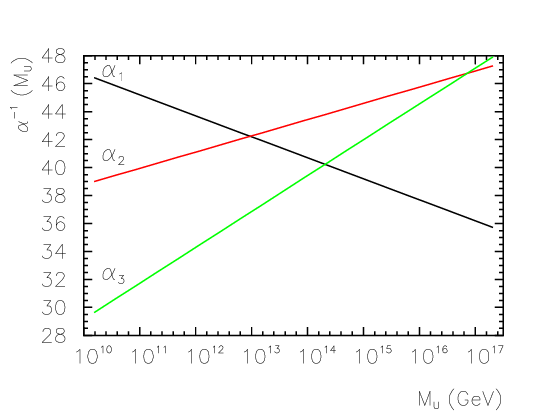
\includegraphics[width=0.8\textwidth]{figures/01-SM-03-SM/qcd/Running-couplings-in-the-standard-model.png}
	\caption{The running of the inverse strength of the SM coupling constants, with the strong coupling constant (\SU[3]) in green, weak (\SU[2]) in red, and electromagnetic (\UU[1]) in black, reproduced from Ref.~\cite{Dias2004}.}
	\label{fig:01_qft_running}
\end{figure}

We see firstly that the electromagnetic interaction strength increases with energy scale.
Physically, this is understood through the \textit{vacuum polarization} via virtual electron-positron pair creation, which ``screen'' the electric charges of real particles more effectively at longer distances, thereby weakening the force.\footnote{Interestingly, QED has a Landau pole: a finite value of the energy scale for which the interaction strength is infinite. However, this value is so high ($10^{286} \GeV$) as to have no practical consequence, and likely points to the breakdown of perturbation theory, that is used to derive the running coupling, at such a scale.}

A notable, Nobel-prize winning, 1973 result of Frank Wilczek, David Gross, and David Politzer, however, was an inverse dependence on energy for non-abelian gauge theories~\cite{Politzer:1973fx, Gross:1973id}, as shown for the \SU[2] and \SU[3] couplings in Figure~\ref{fig:01_qft_running}.\footnote{Technically, this depends on the gauge group and the number of fermions in the theory; for both the weak and strong forces, this number is sufficiently small (see e.g. Peskin and Shroeder~\cite{Peskin:1995ev} Chapter 16).}
This phenomenon is called \textit{asymptotic freedom}, as in the high energy limit the theory is effectively one of free particles.
It is a notable feature of the strong force, as will be discussed in Chapter~\ref{sec:01_sm_qcd}.


\section{The ABEGHHK (Higgs) mechanism}
\label{sec:01_qft_higgs}

As highlighted in the previous section, gauge bosons in pure Yang-Mills theories are massless.
This is in conflict, however, with the short observed range of the weak force, implying massive mediatory bosons.
To resolve this, a series of work in the early 1960s by Anderson, Brout, Englert, Guralnik, Hagen, Higgs, and Kibble (ABEGHHK) yielded a mechanism to give mass to the gauge bosons without violating gauge invariance~\cite{Anderson:1963pc, Englert:1964et, Higgs:1964pj, Guralnik:1964eu}, based on the concept of \textit{spontaneous symmetry breaking} developed by Nambu~\cite{Nambu:1961tp, Nambu:1961fr} and others.

By 1970, Glashow, Salam, Weinberg and others were able to use this mechanism to formulate a combined theory of weak and electromagnetic interactions, known as ``electroweak'' or Weinberg-Salam theory~\cite{Glashow:1959wxa, Salam:1968rm, Weinberg:1967tq}.
Electroweak unification has been one of the most significant breakthroughs in theoretical physics with several Nobel prizes cumulatively awarded for these developments.

In this section we outline the ABEGHHK mechanism --- commonly (but reductively) referred to as the ``Higgs mechanism'' --- first for an abelian gauge theory in Section~\ref{sec:01_qft_higgs_abelian} and then for non-abelian gauge theories~\ref{sec:01_qft_higgs_nonabelian} like the SM.

\subsection{The abelian Higgs mechanism}
\label{sec:01_qft_higgs_abelian}

The Higgs mechanism is based on the idea of spontaneous symmetry breaking (SSB), where the ground states of a physical system violate the overall symmetry.
The classic example is the so-called ``sombrero'' potential for a complex scalar field $\phi$:
\begin{equation}
	\label{eq:01_qft_higgs_potential}
	V(\phi) = -\frac{\lambda}{2}(\abs{\phi}^2 - v^2)^2,
\end{equation}
for constants $\lambda$ and $v$, shown in Figure~\ref{fig:01_qft_higgs_potential}.
The potential has is symmetric under a \UU[1] transformation of $\phi \rightarrow e^{i\alpha}\phi$, but any specific ground state of $\abs{\phi} = v$ will break this symmetry, as shown in the figure.
SSB is a crucial concept in physics, with several applications in condensed matter and particle physics, including chiral symmetry breaking in QCD (see e.g. Tong SM~\cite{TongSM} Chapter 3.2).

\begin{figure}[ht!]
	\centering
	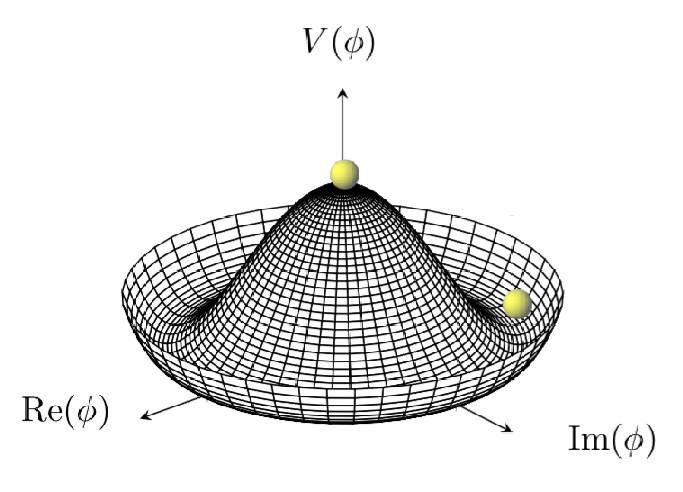
\includegraphics[width=0.7\textwidth]{figures/01-SM-02-QFT/sombrero_potential.png}
	\caption{The ``sombrero'' potential for the Higgs field, reproduced from Ref.~\cite{Duff:2020wmn}.
	An initial state and a ground state breaking the \UU[1] symmetry are represented by the green balls at the top and bottom of the potential, respectively.}
	\label{fig:01_qft_higgs_potential}
\end{figure}

The Higgs mechanism is an application of SSB to \textit{gauge} symmetries.
The interpretation here of SSB a bit fiddly since, as emphasized above, gauge symmetries are not physical and cannot be spontaneously broken;\footnote{This is an implication of Elitzur's theorem~\cite{Elitzur:1975im}.} what actually breaks is the corresponding \textit{global} symmetry, as we outline below.

Consider our QED Lagrangian for a complex scalar field $\phi$ with the above potential:
\begin{equation}
	\label{eq:01_qft_higgs_lagrangian}
	\mathcal L = -\frac{1}{4}F_{\mu\nu}F^{\mu\nu} + (D_\mu\phi)^\dagger D^\mu\phi + \frac{\lambda}{2}(\abs{\phi}^2 - v^2)^2.
\end{equation}
As before, this Lagrangian possesses a \UU[1] gauge symmetry; however, this symmetry is ``broken'' by a particular ground state $\phi = v e^{i\delta}$ (we can take $\delta = 0$ WLOG).
The fluctuations around the ground state can be parametrized as:
\begin{equation}
	\label{eq:01_qft_higgs_fluctuations}
	\phi(x) = (v + \sigma(x))e^{i\theta(x)},
\end{equation}
where $\sigma$ and $\theta$ are two real fields.
Plugging this into the Lagrangian gives us:
\begin{equation}
	\label{eq:01_qft_higgs_fluctuations_lagrangian}
	\mathcal L = -\frac{1}{4}F_{\mu\nu}F^{\mu\nu} + \partial_\mu\sigma \partial^\mu\sigma + (v + \sigma)^2(\partial_\mu\theta - e A_\mu)(\partial^\mu\theta - e A^\mu) - \lambda(2v^2\sigma^2 + 2 v\sigma^3 + \frac{\sigma^4}{4}).
\end{equation}
We see first that $\sigma$ can be interpreted as a normal scalar quantum field, with a quadratic mass term with $m_\sigma^2 = 2\lambda v^2$.
The $\theta$ term is a bit more unusual;\footnote{In a non-gauge-theory, the $\theta$ field would be considered a massless ``Goldstone boson'' resulting from the spontaneously breakdown of the symmetry.}
it only appears in the combination $\partial_\mu\theta - e A_\mu$.
Hence, we can simply redefine the gauge field as $A_\mu' \equiv A_\mu + \frac{1}{e}\partial_\mu\theta$, allowing it to ``absorb'' this DoF.
Note that this takes the form of a gauge transformation of $A_\mu$ and thus does not affect the field strength tensor $F_{\mu\nu}$.
The resulting Lagrangian is then:
\begin{equation}
	\label{eq:01_qft_higgs_fluctuations_lagrangian_final}
	\mathcal L = -\frac{1}{4}F_{\mu\nu}F^{\mu\nu} + \partial_\mu\sigma \partial^\mu\sigma + e^2(v + \sigma)^2A_\mu'A^{'\mu} - \lambda(2v^2\sigma^2 + 2 v\sigma^3 + \frac{\sigma^4}{4}),
\end{equation}
where we now have a mass term for the ``gauge boson'', $m_A^2 = 2e^2 v^2$!

\subsection{The non-abelian Higgs mechanism}
\label{sec:01_qft_higgs_nonabelian}

There is an analogous mechanism for a non-abelian gauge symmetry, as in the SM.
One crucial difference is that the symmetry may only partially break from the gauge group $G$ to a subgroup $H$ (for example from \SU[2] to a \UU[1]).
In this case, the gauge bosons corresponding to the generators of $G$'s broken symmetries acquire mass as above, while the generators of $H$ remain massless Goldstone bosons; as we will see in Chapter~\ref{sec:01_sm_ew}, in the SM these correspond to the massive $W^\pm$ / $Z$ bosons and the massless photon, respectively.
See e.g. Tong SM~\cite{TongSM} Chapter 2.3.3 for an example.


% \section{Brief encounters with renormalization}
% \label{sec:01_qft_renormalization}

%  - perturbation theory leads to infinite integrals at high orders, theory is considered renormalizable if these infinities are canceled or made finite by imposing a cut-off energy scale beyond which the theory is not valid
%  - implicitly, this means that physical parameters of the theory are not fixed, but depend on the energy scale at which they are measured --- the coupling constants, in particular, are considered to "run" with the energy scale.
